%% ****** Start of file aiptemplate.tex ****** %
%%
%%   This file is part of the files in the distribution of AIP substyles for REVTeX4.
%%   Version 4.1 of 9 October 2009.
%%
%
% This is a template for producing documents for use with 
% the REVTEX 4.1 document class and the AIP substyles.
% 


\documentclass[aip,graphicx]{revtex4-1}
\usepackage{graphicx}
\usepackage{longtable}
\usepackage[version=3]{mhchem} % Formula subscripts using \ce{}
\usepackage[T1]{fontenc}       % Use modern font encodings
\usepackage{amsmath}
\usepackage[dvipsnames]{xcolor}
% NB added command for in line cite
%\newcommand{\onlinecite}[1]{\hspace{-1 ex} \nocite{#1}\citenum{#1}} 
%\documentclass[aip,reprint]{revtex4-1}

\draft % marks overfull lines with a black rule on the right

\begin{document}

% Use the \preprint command to place your local institutional report number 
% on the title page in preprint mode.
% Multiple \preprint commands are allowed.
%\preprint{}

\title{Velocity Map Imaging Spectroscopy of C$_2$H$^-$ and C$_2$D$^-$: a benchmark study of vibronic coupling interactions}


\author{Benjamin~A.~Laws}
\email{b.laws@unsw.edu.au}
\affiliation{School of Chemistry, University of New South Wales, Sydney NSW 2052, Australia}
\affiliation{Research School of Physics, The Australian
	National University, Canberra ACT 2601, Australia}
\author{Zachariah~D.~Levey} 
\affiliation{School of Chemistry, University of New South Wales, Sydney NSW 2052, Australia}
\author{Andrei Sanov}
\affiliation{Department of Chemistry and Biochemistry, The University of Arizona, Tucson, Arizona 85721, United States}
\author{John F. Stanton}
\affiliation{Department of Chemistry, University of Florida, Gainesville, Florida 32611, United States}
\author{Timothy~W.~Schmidt} 
\affiliation{School of Chemistry, University of New South Wales, Sydney NSW 2052, Australia}
\author{Stephen~T.~Gibson}
\affiliation{Research School of Physics, The Australian
	National University, Canberra ACT 2601, Australia}




\date{\today}

\begin{abstract}
High-resolution velocity-map imaged photoelectron spectra of the ethynyl anions C$_2$H$^-$ and C$_2$D$^-$ are measured at photon wavelengths between $355-266$~nm, to investigate the complex interactions between the close lying $\tilde{X} ^2\Sigma^+$ and $\tilde{A} ^2\Pi$ electronic states. An indicative kinetic energy resolution of 0.4\%, together with full angular dependence of the fast electrons, provides a detailed description of the vibronically coupled structure. It is demonstrated that a modest quadratic vibronic coupling model, parametrized by the quasidiabatic ansatz, is sufficient to accurately recreate all of the observed vibronic interactions. Simulated spectra are shown to be in excellent agreement with the experimental data, verifying the proposed model, providing a framework that may be used to accurately simulate spectra of larger C$_{2n}$H monohydride carbon chains. New spectral assignments are supported by experimental electron anisotropy measurements and Dyson orbital calculations.
\end{abstract}

\pacs{}

\maketitle 

\section{Introduction}
Carbon monohydrides C$_{2n}$H, are a class of linear radicals that play an important role in combustion and interstellar chemistry~\cite{kie90,kie92,bou96,wil91,vui01}. These carbon chains have been observed in many interstellar environments, including planetary atmospheres~\cite{vui01,wil03,dob16}, comets~\cite{jac96}, dark clouds~\cite{ziu82,gup09}, and during heavy star formation~\cite{beu08,jia15}. Due to their relatively high abundance in a variety of astronomical conditions, they are believed to be promising candidates for Diffuse Interstellar Band (DIB) carriers~\cite{dou77,ful93,wat94,ful00,sch05,gup09}. The corresponding anions C$_{2n}$H$^-$ are also believed to play an important role in interstellar chemistry~\cite{mil17,gup09}. C$_6$H$^-$ was the first negative ion detected in space, after it was observed in two distinct interstellar molecular clouds IRC+10216 and TMC-1 in 2006~\cite{mcc06}. More recently, anions C$_4$H$^-$~\cite{cer07} and C$_8$H$^-$~\cite{bru07,rem07} have also been detected in a range of environments, including dark clouds~\cite{cor13}, prestellar cores,~\cite{sak10} and prostellar envelopes~\cite{sak07}.

Chain growth of the C$_{2n}$H radicals occurs predominately through acetylene addition,~\cite{wil03}
\begin{equation}
\text{C}_{2n}\text{H} + \text{C}_2\text{H}_2 \rightarrow \text{C}_{2n+2}\text{H}+\text{H}_2.
\label{eq:1}
\end{equation}
Conversely, the formation of anions in space is believed to be driven by radiative electron attachment, charge transfer, and dissociative electron attachment. Current astrochemical modelling of interstellar clouds, such as IRC+10216, typically underestimate the observed abundances of CH$_4^-$ ~\cite{mil17,cor13,her08}. Therefore, it has been proposed that ion-neutral reactions
\begin{equation}
\text{C}_{2n}\text{H}^- + \text{C}_2\text{H}_2 \rightarrow \text{C}_{2n+2}\text{H}^- + \text{H}_2
\label{eq:2}
\end{equation}
may be significant chain growth mechanisms that should be included in astrochemical models~\cite{mil17,bas19}. Studies of the extraterrestrial planetary atmosphere of Saturn's moon Titan suggest that both C$_2$H and C$_2$H$^-$ play an important role in the atmospheric chemistry~\cite{dob16,vui09,des17,vri18}. Many reaction pathways involving the C$_2$H$^-$ have been proposed, including reactions with C$_2$H$_2$ and HCN. 

Our knowledge of interstellar chemistry relies critically on theory, to provide a link between astronomical observations and terrestrial laboratory studies. Microwave spectroscopy has successfully been used in this fashion to identify a large number of molecules in the interstellar medium (ISM). However for some species, particularly those with low abundances or no dipole moment, UV/vis spectroscopic methods are required for identification~\cite{mai97}. This creates a challenge for theory, as electronic spectral calculations are more difficult than those employed for pure rotational spectra, particularly when vibronic coupling effects are present as they can be exceedingly difficult to model~\cite{for10}.

These considerations may be explored by examining some of the smallest carbon monohydrides. The ethynyl radical C$_2$H may appear to be a simple linear triatomic molecule. However the electronic spectrum is complicated by the presence of the close-lying ground $^2\Sigma^+$ and first excited $^2\Pi$ surfaces, which are only separated by $\sim3,700~$cm$^{-1}$~\cite{cur85,tar03}. The interaction of these surfaces produces a complex vibronic spectrum around the $\tilde{A}^2\Pi$ state, where the $\tilde{X}-\tilde{A}$ origin is spread over multiple admixed vibronic levels. In C$_4$H the $^2\Sigma^+$ and $^2\Pi$ states are nearly degenerate, resulting in even stronger coupling~\cite{zho07b}, while in C$_6$H and C$_8$H the ordering of the states swaps, with a ground $^2\Pi$ state and a low lying excited $^2\Sigma^+$ state~\cite{lin99,tay98}. Consequently, understanding the vibronic coupling interactions between the $^2\Sigma^+$ and $^2\Pi$ surfaces is essential in order to accurately model the role these radicals (and their corresponding anions) are likely to play in the interstellar chemistry discussed above, and to guide the search for possible DIB carriers.

C$_2$H is reported to be one of the most abundant molecules in the ISM, and is the most thoroughly studied of the C$_{2n}$H species~\cite{wil91,hei99,for10}. Many different experimental techniques have been employed to help understand the complexities of the vibronic spectrum, including electron spin resonance~\cite{coc64,jin85}, laser magnetic resonance~\cite{bro88,pfe96,sch98}, microwave and millimeter wave spectroscopy~\cite{sas81,got83,end89,mul00}, infrared (matrix isolation~\cite{she87,jac87,for95} and Fourier Transform emission~\cite{ver88}) spectroscopy, laser induced fluorescence spectroscopy~\cite{hsu93,hsu95,chi99} and photoelectron spectroscopy of the negative ion~\cite{erv91,tay98,zho07}. Zhou~\emph{et al.} measured photodetachment of C$_2$H$^-$ and C$_2$D$^-$ to both the $\tilde{X} ^2\Sigma^+$ and $\tilde{A} ^2\Pi$ surfaces using slow electron velocity-map imaging (SEVI), which revealed detailed structure around the $\tilde{A} ^2\Pi$ state origin~\cite{zho07}. Comparison with calculations by Tarroni and Carter~\cite{tar03} resulted in detailed spectral assignments, however this was limited by the suppression of $p-$wave structure near threshold.

\subsection{Vibronic Coupling Interactions}
The complex spectral structure observed near the $\tilde{A}^2\Pi$ state origin in previous experiments may be understood by considering the $v_2$ bending vibrational mode. To account for the degeneracy of this mode, the vibronic quantum number $\ell_i$ may be introduced, representing the angular momentum associated with the bending motion. This may take a value of $\ell_i = v_i, v_i-2, v_i-4,\dots,1$ or $0$, where $v_i$ is the quantum of bending excitation. In the Born-Oppenheimer approximation, different vibronic energy levels $\ell_i$ are degenerate, however in cases with strong rovibronic coupling, this degeneracy in $\ell_i$ is lost. 

In C$_2$H the loss of degeneracy creates a Renner-Teller (RT) pair in the excited state, where the usually degenerate $\Pi$ surfaces separate to form two non-degenerate electronic states $\Pi^+ (2A')$ and $\Pi^-(1A'')$. This involves separating a single potential energy surface (V) into two distinct but coupled surfaces (V$^+$) and (V$^-$). Due to the strong coupling along the linear axis between the electronic and vibration angular momenta of the $2A'$ and $1A''$ components of the $^2\Pi$ state, stationary states cannot be explicitly assigned to either of the $\Pi^+(2A')$ or $\Pi^-(1A'')$ electronic surfaces. Instead, they exist as a combination of both states. Due to the close lying nature of the ground {$\tilde{X} ^2\Sigma^+$} and excited {$\tilde{A} ^2\Pi$} electronic states, which are only separated by $\sim3700~$cm$^{-1}$, a pseudo Jahn-Teller effect is also observed. In the case of C$_2$H this is seen as coupling between the ground $\Sigma^+(1A')$ and excited $\Pi^+(2A')$ states, induced by the bending motion of $v_2$. The ground state only couples to one member of the Renner-Teller pair $\Pi^+(2A')$, as the other state $\Pi^-(1A'')$ has incompatible symmetry. This results in the complex vibronic structure observed for the $\tilde{A}^2\Pi$ electronic state, with contributions from three coupled surfaces $\Sigma^+(1A'),$ $\Pi^+(2A'),$ and $\Pi^-(1A'')$.

These interactions spread the electronic origin of the $\tilde{A}\,^2\Pi$ state over several vibronic levels. Therefore, instead of assigning a defined origin, the peaks observed in experimental spectra may be assigned to coupled admixtures of vibronic transitions involving the three potential energy surfaces,
\begin{equation}
\Psi_f = \sum_\xi \psi_e^\xi \sum_k C_{fk}^\xi\phi_{fkm}^\xi,
\label{eq:3} 
\end{equation}
where $\psi_e^\xi$ is the diabatic electronic wavefunction, and $\phi_{fkm}^\xi$ is the spin-rovibrational wavefunction. $\xi$ represents the electronic states used in the expansion ($\xi=\Sigma^+(1A'),~\Pi^+(2A'),~\Pi^-(1A'')$).

C$_2$H has received extensive theoretical attention in an attempt to interpret the experimental results~\cite{per90,per91,per91b,per91c,per92,car00,tar03,tar04,for10,sta21,gul21}. This includes the variational method of Tarroni and Carter, which has been used to calculate a multitude of admixed vibronic levels in C$_2$H. A depiction of the three interacting potential energy surfaces in Eq.~(\ref{eq:3}), generated from the variational parameters of Ref~\onlinecite{tar03}, is shown in Fig.~\ref{fig:1}. This illustrates the loss of degeneracy for the doublet $^2\Pi$ surfaces along the CCH bending coordinate, due to the Renner-Teller and pseudo Jahn-Teller interactions. From these surfaces more than 100 possible C$_2$H vibronic states have been calculated, up to 10,000~cm$^{-1}$ above the $\tilde{X} ^2\Sigma^+$ origin~\cite{tar03}. However, assigning experimental spectra has remained a challenge, partly due to the large number of calculated levels, providing multiple options for each experimentally observed transition. The complexity of the variational approach also limits the extension of this method to larger C$_{2n}$H chains.

In this work we demonstrate that the construction of a quasidiabatic Hamiltonian allows the strength of vibronic interactions between coupled surfaces near a conical intersection to be estimated, sufficient to accurately simulate electronic and vibronic spectra. Anion HR-PEI spectroscopy maps both of the $^2\Sigma^+$ and $^2\Pi$ surfaces on an equal footing from the anion $\tilde{X}^1\Sigma^+$ state, allowing a direct comparison with the \emph{ab-initio} modelling. This is combined with experimental anisotropy measurements and Dyson orbital analysis to examine the vibronic symmetry of each observed transition to verify spectral assignments.

\begin{figure}
	\centering
	\includegraphics[width=0.5\textwidth]{figures/Fig1}
	\caption{Adiabatic potential energy surfaces of $\tilde{X}^2\Sigma^+$, $\tilde{A}^2\Pi^-$, and $\tilde{A}^2\Pi^+$ states, calculated using the parameters calculated by Tarroni and Carter~\cite{tar03}.}
	\label{fig:1}
\end{figure}


\section{Methods}
\subsection{Experimental Procedure}
Details of the HR-PEI spectrometer are given in Refs.~\onlinecite{cav07} and~\onlinecite{dev17}. Briefly, ethynyl ions C$_2$H$^-$ and C$_2$D$^-$ were produced in a pulsed-jet discharge of pure ethylene (C$_2$H$_4$/C$_2$D$_4$) gas, and subsequently mass isolated over a 2m-long time of flight region~\cite{ded01}. Electrons were detached using a tuneable Continuum Sunlite Ex Optical Parametric Oscillator (OPO) pumped with the third harmonic (355~nm) of a Nd:YAG laser. Higher electron counts were also obtained with the direct use of the third and fourth harmonics (266~nm) from the Nd:YAG laser. The detached electrons are mapped onto a micro-channel plate detector using a modified Velocity Map Imaging (VMI) lens. Each detachment event is imaged by a 2048x2048 monochrome CCD camera (PCO 2000), with each frame transferred to a computer within the 10Hz repetition rate of the laser and processed in real time to identify electron events, centroiding each position to a subpixel accuracy.

The resulting velocity-map image is centred and then circularized by an angular dependent-radial scaling determined by comparing adjacent radial slice intensity profiles~\cite{gas17}. An inverse Abel transformation of the velocity-map image, based on the algorithm of Hansen and Law~\cite{han85,hic19}, returns a slice image of the 3D electron source distribution. Absolute energy calibration of the photoelectron spectra is achieved using published measurements of species, including C$_2^-$~\cite{law19b} and NO$_2^-$~\cite{law19}, that have been studied under similar conditions and photon energies as those used for the C$_2$H$^-$ measurements.

%--------------------------------------------------------------------


\subsection{Computational Details}
Quantum chemical computations were preformed using the CFOUR computational package~\cite{dev20}. The equation-of-motion ionized-potential coupled-cluster singles, doubles, and triples (EOM-IP-CCSDT) level of theory with an atomic natural orbital basis set of quadruple-zeta quality (ANO2) was used on a closed-shell anionic reference to perform geometry optimisations and frequency calculations (including 1h + 2h1p + 3h2p excitations~\cite{mat16}). EOM is a highly accurate and robust framework that provides access to different types of target electronic states, including ionized states, making it well suited to the study of photodetachment~\cite{gul21b,and22,bar07}. The linear diabatic coupling constants were calculated analytically at the EOM-IP-CCSD/ANO2 level.

Dyson orbitals, that are used to analyse the experimental electron anisotropy, were generated using Q-Chem software~\cite{sha15} at the EOM-CCSD/aug-gg-pVTZ level. Anisotropy parameters were then calculated using the ezDyson software of Gozem and Krylov~\cite{goz22}.

\subsection{The Quasidiabatic Ansatz} 
In order to guide spectral assignment of C$_2$H and future astronomical searches for other C$_n$H radicals, transition intensities are required. However, due to the strong vibronic coupling interactions, transition intensities can not be obtained via simple Franck-Condon calculations based on quantum chemistry methods. To account for these interactions, the photoelectron spectrum of the C$_2$H$^-$ anion is simulated, in this work, using a quasidiabatic Hamiltonian of the type introduced by Koeppel, Domcke and Cederbaum (KDC).~\cite{kou84,dom81} In this approach, the Hamiltonian is represented in a basis of quasidiabatic (slowly varying) electronic  states for which the kinetic energy operator can be assumed diagonal.~\cite{pac93} For C$_2$H, the KDC Hamiltonian comprises three states - the two components of the $^2\Pi$ state and the ground $^2\Sigma^+$ state - and is then projected onto a vibrational basis, usually chosen as a direct product of harmonic oscillators. Diagonalization of the corresponding matrix yields the molecular states (which are given in terms of a Born-Huang expansion), and the squared projections of the corresponding eigenvectors onto the ground state of the anion yield the relative intensities. The latter is true only if the photodetachment cross sections for the $^2\Sigma^+$ and $^2\Pi$ states are assumed equal, but different cross sections of the two states can be incorporated by scaling the intensities of states according to their (vibronic) symmetry.~\cite{sta11} 

Details of the construction and parametrization of KDC Hamiltonians can be found elsewhere in the literature,~\cite{sta21,ich06,ich08,ich09,wei17} and the procedure followed will be discussed here only briefly. The present calculations use the so-called quadratic vibronic coupling (QVC) model.~\cite{ich06} For the system at hand, the QVC model Hamiltonian  assumes the following form
\begin{align}
H &= T_n1+V,\\
V &= \bordermatrix{ & X & A(a') & A(a'') \cr
	X &\substack{\Delta_0^X+F_1^Xq_1+F_3^Xq_3+\\ 
		\frac{1}{2} \sum_{ij}F^X_{ij}q_iq_j}& \lambda q_{2a} & \lambda q_{2b} \cr
	A(a') & \lambda q_{2a} & \substack{\Delta^A_0+F^A_1q_1+F^A_3q_3\\+\frac{1}{2}\sum_{ij}F^A_{ij}q_iq_j+\\\frac{1}{2}\eta(q_{2a}^2-q_{2b}^2)} & \eta q_{2a}q_{2b} \cr
	A(a'') & \lambda q_{2b} & \eta q_{2a}q_{2b} & \substack{\Delta_0^A+F_1^Aq_1+F_3^Aq_3\\+\frac{1}{2}\sum_{ij}F_{ij}^Aq_iq_j\\-\frac{1}{2}\eta(q_{2a}^2-q_{2b}^2) } } \qquad
\label{eq:5}
\end{align}
where the summations run over the dimensionless normal modes ($q_i$) that serve as the coordinate system for the problem.~\cite{sta21,car00} For convenience, the latter are chosen to be those of the anion, which considerably facilitates calculation of the spectral intensities.  In Eq.~(\ref{eq:5}), the diagonal terms of V (excluding those that carry the Renner-Teller coupling constant $\eta$) represent the quasidiabatic potential energy surfaces of the $^2\Sigma^+$ state, and the two components of the $^2\Pi$ state, chosen here as those in which the unpaired electron lies within or is perpendicular to an arbitrarily chosen plane, designated as A(a$'$) and A(a$''$), respectively. $\Delta_0^X$ is the separation of the anion and $^2\Sigma^+$ states at the origin of the coordinate system (the vertical electron detachment energy), and $\Delta_0^{A}$ is the gap between anion and $^2\Pi$ states at the same geometry.   

For the modes of $\sigma$ symmetry ($q_1$ and $q_3$), the diabatic forces ($F_i$) and force constants ($F_{ij}$) coincide with those of the adiabatic potential energy surfaces.   However, for the bending mode, the diabatic (F$_{22}$) and adiabatic (f$_{22}$) force constants differ, and the parametrization is somewhat more involved.   For each component of the $^2\Pi$ state, either the 2a or 2b component of the bending vibration will maintain the A$'$ electronic symmetry that is needed to couple with the $^2\Sigma^+$ state.  Designating these as 2a for the A(a$'$) state and 2b for the A(a$''$) state (as is implicit in Eq.~\ref{eq:5}), the diabatic force constants for the bending mode in the $^2\Sigma^+$ and $^2\Pi$ states can be written as 
\begin{align}
F_{22}^X &= f_{22}^X+\frac{2\lambda^2}{(\Delta_0^A-\Delta_0^X)}\\
F_{22}^A &= f_{2a2a}^{A(a')}-\frac{2\lambda^2}{(\Delta_0^A-\Delta_0^X)}-\eta
\label{eq:7}
\end{align}
where the Renner-Teller interaction strength ($\eta$) is determined from 
\begin{equation}
\eta = \frac{1}{2}\left[ f_{2a2a}^{A(a')}-f_{2b2b}^{A(a')}-\frac{2\lambda^2}{(\Delta_0^A-\Delta_0^X)}\right]
\label{eq:8}
\end{equation}
once the interstate coupling ($\lambda$ which is calculated analytically in this work) is known.


\section{Results and Analysis}
An illustrative velocity map image containing $\sim$4 million electrons, collected from 355~nm (3.49~eV) photodetachment of C$_2$H$^-$ is shown in Fig.~\ref{fig:2}(a), and for C$_2$D$^-$ detachment under the same conditions in Fig.~\ref{fig:2}(b). In both images the laser polarisation is aligned along the vertical axis, and electrons are distributed radially according to their speed, with slow electrons near the image center, and fast electrons located towards the outer edge. Due to the relatively large C$_2$H electron affinity (EA) of 2.969~eV~\cite{erv91}, photodetachment at 355~nm produces photoelectrons with small (< 0.5~eV) kinetic energies, resulting in high electron velocity resolution, with transition widths varying from 21~cm$^{-1}$ (around 24,000~cm$^{-1}$) to only 7~cm$^{-1}$ (near 28,000~cm$^{-1}$). Despite the photodetachment energy being close to threshold, detachment to both the $\tilde{X} ^2\Sigma^+$ and $\tilde{A} ^2\Pi$ electronic states is observed due to the low Term energy $\sim 3,700~$cm$^{-1}$. The faster electrons, on the outer edge of Figs.~\ref{fig:2}(a) and (b), correspond to C$_2$H$(\tilde{X}\,^2\Sigma^+)+e^- \leftarrow $C$_2$H$^-(\tilde{X}\,^1\Sigma^+)+h\nu$ photodetachment, and are preferentially distributed around the poles of the image, indicative of a positive electron anisotropy parameter. Conversely the angular distribution of the slower electrons, near the center of Figs.~\ref{fig:2}(a) and (b), is skewed towards the equator, indicative of a negative anisotropy parameter~\cite{buc70}. These electrons may be assigned to photodetachment to the first excited state C$_2$H$(\tilde{A}\,^2\Pi)+e^- \leftarrow $C$_2$H$^-(\tilde{X}\,^1\Sigma^+)+h\nu$.

\begin{figure}
	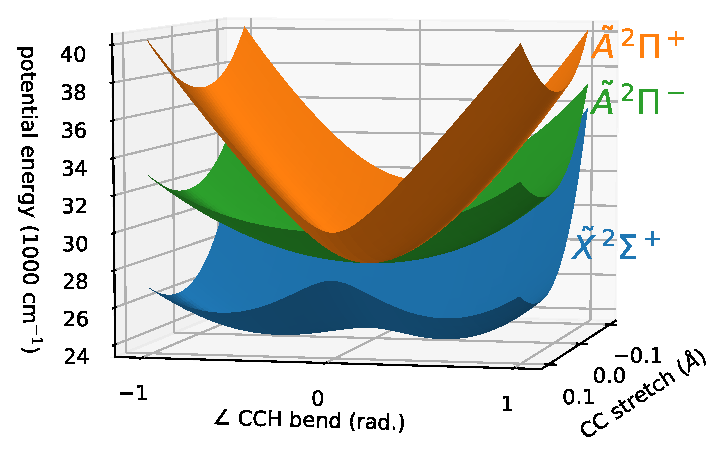
\includegraphics[width=0.8\textwidth]{figures/Fig2}
	\caption{(a) Velocity map image of electrons from C$_2$H$^-$ photodetachment at 355~nm. (b) Velocity map image of C$_2$D$^-$ at 355~nm. Both images contain $\sim4$ million electrons. (c) Comparison of the corresponding 355~nm photoelectron spectra for C$_2$H$^-$ and C$_2$D$^-$. Structure below $\sim 27,000~$cm$^{-1}$ is associated with the ground state $\tilde{X} ^2\Sigma^+$, while structure above  $\sim 27,000~$cm$^{-1}$ is largely due to the excited neutral $\tilde{A} ^2\Pi$ state.}
	\label{fig:2}
\end{figure}

The velocity-map images of Fig.~\ref{fig:2} were inverted using the Abel inversion methods detailed in PyAbel~\cite{hic19} to extract the corresponding photoelectron spectra, presented in Fig.~\ref{fig:2}(c). The structure below $27,000~$cm$^{-1}$ in binding energy, corresponding to the $\tilde{X} ^2\Sigma^+$ surface, is similar for both C$_2$H$^-$ and C$_2$D$^-$ detachment. They are dominated by the origin transition, shifted by $\sim10~$cm$^{-1}$ in the deuterated spectrum, with progressions involving the v$_2$($\pi$) bending and v$_3$($\sigma$) CC stretch vibrational normal modes. This structure also includes transitions involving an odd quanta of v$_2$ bending excitation ($2^{n+1}$) which are totally forbidden within the Franck-Condon approximation. The presence of these transitions in the spectra is an indicator of Herzberg-Teller (HT) vibronic coupling between the ground $^2\Sigma^+$ and nearby excited $^2\Pi$ electronic surfaces, as
\begin{equation}
\Sigma^+ \otimes \pi = \Pi. 
\label{eq:9}
\end{equation}

At binding energies above $\sim27,000~$cm$^{-1}$ in Fig.~\ref{fig:2}(c), near the $\tilde{A}^2\Pi$ state origin, significant differences are observed between the C$_2$H$^-$ and C$_2$D$^-$ photoelectron spectra. In C$_2$H$^-$, 5 sharp peaks are observed, spaced by $\sim95~$cm$^{-1}$. However in the deuterated spectrum, one dominant peak is observed near $27,790$~cm$^{-1}$, with 3 weaker peaks centred around $27,360~$cm$^{-1}$. Unlike the structure below $27,000$~cm$^{-1}$ none of these peaks are able to be readily assigned to vibronic transitions, due to the presence of strong coupling interactions between the nearby $\Sigma^+$ and $\Pi$ surfaces.

%--------------------------------------------------

\subsection{Vibronic Coupling Calculations}
The QVC model Hamiltonian (Eq.~\ref{eq:5}) generated in Section II C was employed to calculate the vibronic coupling effects observed in the photoelectron spectra of C$_2$H$^-$ and C$_2$D$^-$ in Fig.~\ref{fig:2}. When the QVC Hamiltonian is diagonalized, the adiabatic states that are used for its parametrization are precisely recovered through terms second order in displacement. The parametrization of the potential in this work was completed using the CFOUR computational package~\cite{dev20} and the quasidiabatic ansatz of Ichino~\emph{et al.}~\cite{ich09} Briefly, the EOM procedure is used to operationally define quasidiabatic states (those that relax according to a well-behaved reference state wavefunction, which is that of the anion level) and the coupling constants are then evaluated as the first derivative of the off-diagonal elements of the electronic Hamiltonian in the basis defined by this representation. Vertical excitation energies ($\Delta_0$), and linear diabatic force and coupling constants between the electronic states of interest were calculated analytically using the highly accurate EOM-IP-CCSDT/ANO2 procedure. The interstate coupling constants ($\lambda$) were calculated analytically at the EOM-IP-CCSD/ANO2 level. All calculated values used to parametrize the KDC potential in Eq.~(\ref{eq:5}) are presented in Table~\ref{tab:1}.

\begin{table}
	\caption{Parameters for the quasidiabatic Hamiltonian Eq.~(\ref{eq:5}) determined using CFOUR and the quasidiabatic ansatz. Units are in cm$^{-1}$.}
	\label{tab:1}

	\begin{tabular}{c | r r r r | r r r r} 
		\hline
		& \multicolumn{4}{c}{C2H} & \multicolumn{4}{c}{C2D}\\
		\hline
		& ~~Anion~~ & ~~$\tilde{X}^2\Sigma^+$~~ & ~~$\tilde{A}^2\Pi (a')$~~ & ~~$\tilde{A}^2\Pi (a'')$~~ & ~~Anion~~ & ~~$\tilde{X}^2\Sigma^+$~~ & ~~$\tilde{A}^2\Pi (a')$~~ & ~~$\tilde{A}^2\Pi (a'')$~  \\
		\hline
		$\Delta_0$ & 0& 22431.21&  26543.67& 26543.67& 0 & 22431.21& 26543.67& 26543.67 \\
		F$_1$ &  0& -211.28& 286.90& 286.90& 0& -596.04& 641.6& 641.6\\
		F$_3$ &  0& -1515.21&  1257.07& 1257.07& 0& -1401.53& 1115.17& 1115.17\\
		F$_{2a}$& 0 & 0& 0& 0& 0& 0& 0&0 \\
		F$_{2b}$&  0& 0& 0& 0& 0& 0& 0&0 \\
		F$_{11}$& 3424.32 &  3487.03& 3482.16& 3482.16& 2611.42&  2636.57& 2681.25& 2681.25\\
		F$_{13}$&  0 & -28.32& 31.46& 31.46& 0& -48.38& 55.40& 55.40\\
		F$_{33}$& 1894.71 & 1830.83& 2042.21& 2042.21& 1792.49&  1747.62& 1914.39& 1914.39\\
		f$_{22}$& 607.09&  87.57& -& -& 481.89&  120.09& -& -\\
		F$_{22}$& 607.09 & 770.78& -& -& 481.89& 620.70& -& -\\
		f$_{2a2a}$& - &- & 1883.48& 658.96& -& -& 1503.88& 473.55\\
		f$_{2b2b}$& - &- & 658.96& 1883.48& -& -& 473.55& 1503.88\\
		F$_{2a2a}$& -& -& 1200.27& 658.96& -& -& 1003.27& 473.55\\
		F$_{2b2b}$& -& -& 658.96& 1200.27& -& -& 473.55& 1003.27\\
		&&&&&&&& \\
		$\lambda$& & & -1185.26& & & & -1014.58& \\
		$\eta$ & & & -270.66& & & & -264.86& \\
		
	\end{tabular}
\end{table}

The photdetachment transitions of C$_2$H$^-$ and C$_2$D$^-$ were calculated using the parameters in Table~\ref{tab:1} and the xsim package of CFOUR~\cite{dev20}. The xsim module projects the Hamiltonian (Eq.~\ref{eq:5}) onto a vibrational basis, which is then diagonalized using Lanczos algorithm to calculate transition energies and intensities that map to the measured photoelectron spectrum. In this simulation the transition moments for the two ionization processes are assumed to be equal. The calculated transitions are shown in Figs.~\ref{fig:3}(a) and (b) alongside the experimental photoelectron spectra measured at 355~nm. Transitions with $\Sigma$ vibronic symmetry are shown in blue and transitions with $\Pi$ symmetry are in orange. The positions of the $\tilde{A} ^2\Pi$ transitions have been shifted by 500~cm$^{-1}$ to account for the EOMIP-CCSDT calculations overestimating the effective Term energy ($\Delta^A_0-\Delta^X_0$ in Table~\ref{tab:1}).

\begin{figure}[th!]
	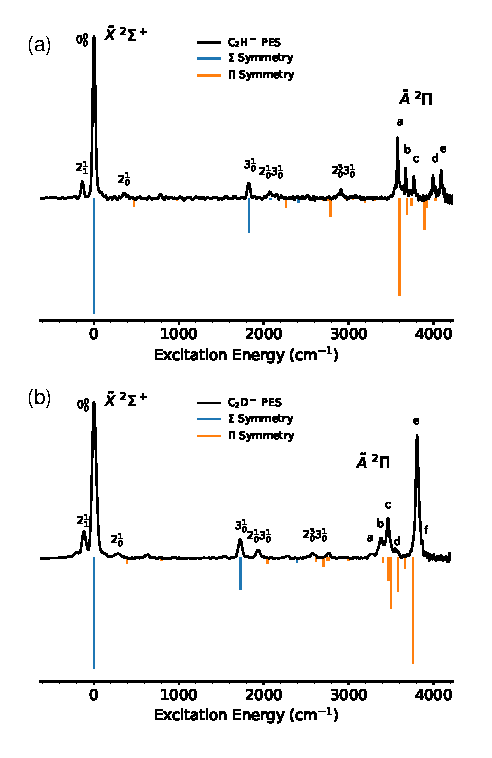
\includegraphics[width=0.6\textwidth]{figures/Fig3}
	\caption{(a) Experimental photoelectron spectrum of C$_2$H$^-$ at 355~nm, compared with the simulated spectrum, calculated using the quasidiabatic ansatz. Transitions with $\Sigma$ symmetry are shown in blue, and those with $\Pi$ symmetry are shown in orange. (b) Experimental photoelectron spectrum of C$_2$D$^-$ at 355~nm, compared to the simulated spectrum. The labelling of peaks near the $\tilde{A}$ origin correspond to transitions identified in Tables~S1 and~S2.}
	\label{fig:3}
\end{figure}

Figure~\ref{fig:3}(a) shows excellent agreement in both the transition positions and intensities between the calculated and experimental C$_2$H$^-$ photodetachment spectra on the $\tilde{X} ^2\Sigma^+$ surface, below $3,600~$cm$^{-1}$. This includes the HT coupled (2$^{n+1}$) transitions with $\Pi$ symmetry, which would normally be missing from a simulation using the standard \emph{ab-initio} approaches. Near the excited state surface (peaks $a-e$ in Fig.~\ref{fig:3}(a)) the experimental data shows that the electronic coupling interactions induce a splitting of the $\tilde{A} ^2\Pi$ state origin over 5 vibronic levels, spaced by $\sim 95~$cm$^{-1}$. This splitting is also observed in the calculated spectrum, which reproduces the 5 prominent transitions in this region. Fig.~\ref{fig:3}(a) shows that the relative intensities between the calculated transitions near $3,700~$cm$^{-1}$ are also in agreement with the experimental data. Peak $d$ is slightly overestimated in intensity, which may in part be due to the variation of photodetachment cross section near threshold, as described by the Wigner threshold law~\cite{wig48}. The simulated spectrum also slightly underestimates the magnitude of the splitting between the vibronic levels, which may be linked to the overestimation of the calculated gap between the $^2\Sigma^+$ and $^2\Pi$ surfaces.

The photoelectron spectrum of C$_2$D$^-$ was also examined using the same approach, with the calculated transitions shown in Fig.~\ref{fig:3}(b) alongside the 355~nm experimental data. Again, there is excellent agreement in the intensity and calculated positions of the transitions on the $\tilde{X} ^2\Sigma^+$ state surface (below $3,600~$cm$^{-1}$ in Fig.~\ref{fig:3}(b)). This includes the HT coupled transitions ($2^1_0,~2^1_03^1_0,~2^3_03^1_0$). Near the $\tilde{A} ^2\Pi$ state origin, deuteration has a large impact on the experimental photoelectron spectrum. Instead of the 5 evenly split levels observed in C$_2$H$^-$ in Fig.~\ref{fig:3}(a), a single dominant peak ($e$) is now observed near $\sim3,845$~cm$^{-1}$ alongside a collection of weaker peaks ($a-d$) centred around 3,400~cm$^{-1}$. Based on the observed spin-orbit splitting measurements from rotationally resolved IR spectra~\cite{yan87,sch98,ste88}, peak $e$ is expected to have significant $\tilde{A} ^2\Pi$ character, with peaks $a-d$ commonly assigned to vibronic levels with predominantly HT coupled $\tilde{X} ^2\Sigma^+$ character~\cite{yan87,hsu95,chi99,wil11}. This suggests that deuteration effectively dampens the coupling interaction between the surfaces, as has been observed in the vinylidene photoelectron spectrum~\cite{dev17}. This is supported by the reduction in the calculated coupling constants $\lambda$ and $\eta$ for C$_2$D$^-$ in Table~\ref{tab:1}.

The calculated transitions in Fig.~\ref{fig:3}(b) reproduce the large change observed experimentally for the deuterated species. The calculated intensity pattern of the vibronic levels around the $\tilde{A} ^2\Pi$ origin also mirrors the experimental data, with a single intense transition observed near peak $e$, and 3 prominent transitions predicted around the experimental peaks $a-d$. The calculated splitting between the levels is also similar, verifying that the proposed QVC model is an accurate method for calculating the vibronic coupling interactions in C$_2$H and C$_2$D.  

\subsection{Excited State Simulation}
To investigate the effects of coupling on the higher excited vibronic levels on the~$\tilde{A} ^2\Pi$ surface, the calculations were compared with the experimental photoelectron spectrum of C$_2$H$^-$ at 266~nm, as presented in Fig.~\ref{fig:4}. Photodetachment at 266~nm (4.66~eV) maps out more of the $\tilde{A} ^2\Pi$ potential energy surface, at the cost of lower electron velocity resolution. Gaussian functions were fitted to the transitions from Fig.~\ref{fig:3}(a) with a kinetic energy dependent FWHM of $\Delta\text{E}/\text{E} = 0.4\%$ ($\Gamma=55-30$~cm$^{-1}$) to match the lower resolution of the experimental data at high electron kinetic energies. By showing the convolved spectrum, the suitability of the QVC model to simulate spectra capable of direct comparison to experimental or astronomical data can be examined. In Fig.~\ref{fig:4} the electronic origin of the $\tilde{A} ^2\Pi$ state (near $\sim3,700~$cm$^{-1}$) is split over 5 vibronic levels, as has been discussed above. A similar effect is also observed for the $3^1_0$ band near $\sim5,400~$cm$^{-1}$, which becomes split over 3 vibronic levels labelled $l$, $n$, and $o$. The calculated spectrum correctly predicts the position and intensity of peaks $n$ and $o$, but appears to strongly underestimate the intensity of peak $l$. Between the $0^0_0$ and $3^1_0$ bands a collection of weaker peaks are also observed ($f-k$). These are assigned to highly excited HT coupled $\tilde{X} ^2\Sigma^+$ transitions ($j,k$), admixed $\tilde{X}-\tilde{A}$ transitions ($h,i$) and pure $\tilde{X} ^2\Sigma^+$ transitions ($f$). Consequently, peak $f$ will possess $\Sigma$ symmetry, and should have a different anisotropy to all of the other dominant transitions above 3,800~cm$^{-1}$. The position and intensity of these highly-excited coupled transitions are well described by the simulated spectrum.

\begin{figure}[th!]
	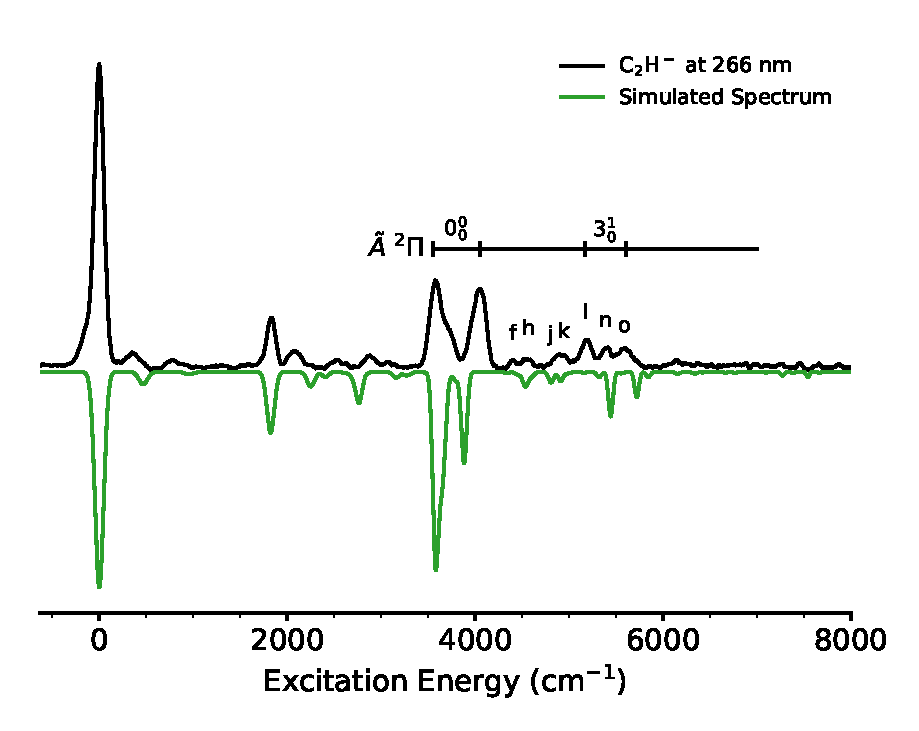
\includegraphics[width=0.6\textwidth]{figures/Fig4}
	\caption{Photoelectron spectrum of C$_2$H$^-$ at 266~nm, showing vibrationally excited $\tilde{A}$ state structure. The simulated spectrum, shown in green, is calculated using the quasidiabatic ansatz, and convolved with a Gaussian function with a kinetic energy dependent FWHM of $\Delta\text{E}/\text{E} = 0.4\%$ ($\Gamma=55-30$~cm$^{-1}$) to match the VMI resolution characteristics.}
	\label{fig:4}
\end{figure}

The results from Figs.~\ref{fig:3} and~\ref{fig:4} confirm that the quasidiabatic approach is able to accurately describe the vibronic interactions between the $^2\Sigma^+$ and $^2\Pi$ surfaces, including deuteration effects. This validates the proposed vibronic interactions, and demonstrates how this method can be employed to decode and assign even complex spectra. While the present calculations invoke a high level of \emph{ab-initio} theory (EOM-IP-CCSDT), the level of parametrization of the vibronic Hamiltonian is relatively simple (QVC model). The approach could be systematically improved with a more elaborate expansion, such as that used in Ref.~\onlinecite{sim12} for the NO$_3$ radical. Applying this approach to similar systems will likely produce reliable predictions for the position and intensity of dominant transitions and help guide the search for these molecules in laboratory experiments and astronomical observations. 

\subsection{Photoelectron Angular Distributions}
Symmetry considerations may be employed to verify the spectral assignments from the calculations above. The quasidiabatic Hamiltonian approach is able to determine the symmetry of each individual vibronic state, either $\Sigma$ or $\Pi$, which may be compared directly to the observed anisotropy of each transition. The velocity-map images from this work (Fig.~\ref{fig:1}) were obtained using a linearly polarized detachment laser. Therefore, the differential cross section of emitted electrons is given by  
\begin{equation}
\frac{\text{d}\sigma}{\text{d}\Omega}=\frac{\sigma_{\text{total}}}{4\pi}[1+\beta P_{2}(\cos\theta)],
\label{eq:10}
\end{equation}
where $\theta$ is the angle between the ejected electron and the (vertical) 
laser polarization, and $P_2$ is the second-order Legendre polynomial. The electron anisotropy parameter $\beta$ provides a quantitative measure of the electron anisotropy, which ranges from -1 to +2, the limits representing purely perpendicular and parallel transitions respectively. Through conservation of angular momentum, $\beta$ may be described in terms of the detachment partial waves, which are linked to the symmetry of the state accessed by photodetachment. This is discussed in detail elsewhere\cite{khu14,law19}, and is only briefly described for the case of C$_2$H$^-$ here. 

Photodetachment to the ground state of C$_2$H $(\tilde{X}\,^2\Sigma^+)$ involves ejecting an electron from an $s-$like $\sigma$ orbital (approximately $5\sigma_g$ in symmetry character), whereas detachment to the excited $\tilde{A}\,^2\Pi$ state occurs from a $p-$like $\pi$ orbital (approximately $1\pi_u$ in character)~\cite{gul21}. Therefore, the electron anisotropies may be described using the mixed $s-p$ model\cite{khu14},
\begin{equation}
\beta_{sp}(\epsilon) = \frac{2(1-\gamma_p)B_1\epsilon + \gamma_p(2A_1^2\epsilon^2-4A_1\epsilon\cos\delta_{2,0})}
{(1-\gamma_p)B_1\epsilon+\gamma_p(1+2A_1^2\epsilon^2)}
\label{eq:11}
\end{equation}
where $\epsilon$ is the electron kinetic energy and $\gamma_p$ is the fraction of $p$ character of the detachment orbital described as,
\begin{equation}
|\psi\rangle = \sqrt{1-\gamma_p}|s\rangle + \sqrt{\gamma_p}|p\rangle.
\label{eq:12}
\end{equation}
$A_1$ and $B_1$ in Eq.~(\ref{eq:11}) are the generalised Hanstorp~\cite{han89} coefficients describing the assumed Wigner-like~\cite{wig48} relative scalings of the radial transition dipole matrix elements for different allowed detachment channels. Specifically, $A_1\epsilon$ describes the energy-dependent ratio of the $p\rightarrow d$ and $p\rightarrow s$ transition amplitudes, while $B_1\epsilon$ corresponds to the $s\rightarrow p$ and $p\rightarrow s$ cross-section ratio~\cite{khu14}. It can be shown that under certain approximations $B_1/A_1 = 8/3$~\cite{san13}. Finally, $\delta_{2,0}$ in Eq.~(\ref{eq:11}) is the phase shift between the $s$ and $d$ partial waves, which in most cases of anion photodetachment is assumed to be small, corresponding to $\cos\delta_{2,0}\approx1$.

From Eq.~(\ref{eq:11}) it can be seen that detachment from a pure $s$ orbital ($\gamma_p=0$) will have a positive anisotropy ($\beta = +2$), whereas detachment from a pure $p$ orbital ($\gamma_p=1$) will have a negative anisotropy for electron kinetic energies $\epsilon < 2/A_1$. Therefore, measuring the anisotropy can help determine the electronic character of each individual transition, which may be compared to the calculated symmetries in Fig.~\ref{fig:3}. For each prominent transition in the photoelectron spectrum of C$_2$H$^-$ in Fig.~\ref{fig:1} the corresponding anisotropy parameter may be calculated by fitting Eq.~(\ref{eq:10}) to a plot of the integrated radial intensity (across the peak) versus angle, as (for a single quadrant of the electron image) the intensity variation is linear in $P_2(\cos\theta)$ with a slope equal to $\beta\times$intercept. This procedure was applied to all of the photoelectron spectra measured in this work, with the energy dependent anisotropy parameters presented in Fig.~\ref{fig:5}(a).


\begin{figure}[th!]
	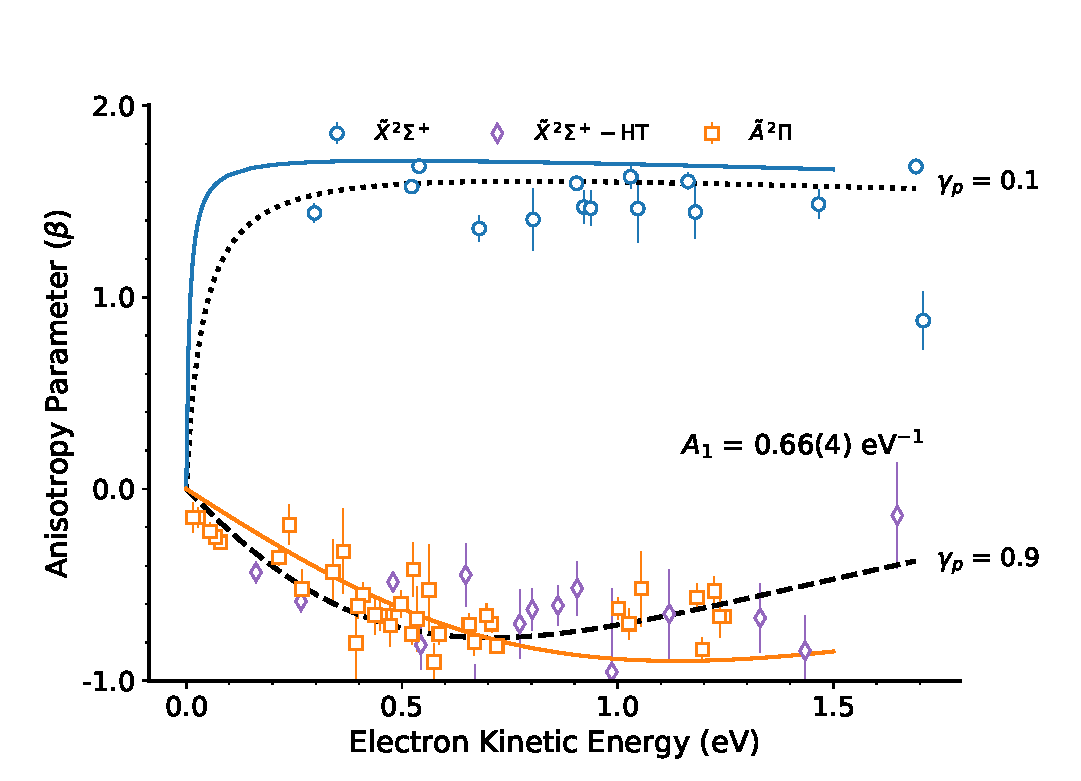
\includegraphics[width=0.8\textwidth]{figures/Fig5}
	\caption{(a) Photoelectron anisotropy parameters, measured for each resolved C$_2$H$^-$ transition, across a range of detachment wavelengths. Allowed ground state transitions $\tilde{X}^2\Sigma^+$ are shown in orange, Herzberg-Teller coupled transitions are shown in purple, and excited state transitions $\tilde{A} ^2\Pi$ are shown in blue. Anisotropy curves for a mixed-$sp$ model (Eq.~\ref{eq:11}) are shown for $\gamma_p=0.1$ and $\gamma_p=0.9$. Anisotropy curves from Dyson orbital calculations for the $\tilde{X}^2\Sigma^+$ and $\tilde{A} ^2\Pi$ transitions are shown in blue and orange respectively. (b) Dyson orbital representation of the $\tilde{X}^1\Sigma^+\rightarrow\tilde{X}^2\Sigma^+$ transition. (c) Dyson orbital representation of the $\tilde{X}^1\Sigma^+\rightarrow\tilde{A} ^2\Pi$ transition.}
	\label{fig:5}
\end{figure}

In Fig.~\ref{fig:5}(a) allowed ground state transitions ($\tilde{X}^2\Sigma^+$) are shown in blue and have a positive anisotropy, as expected for detachment from a $s-$like orbital. Conversely, excited state transitions ($\tilde{A} ^2\Pi$) shown in orange have a negative anisotropy. However, the HT coupled transitions on the $\tilde{X} ^2\Sigma^+$ surface (shown in purple) also have negative anisotropies, due to their $\Pi$ vibronic symmetry. Therefore, the sign $(+/-)$ of $\beta$ can be used to assign each accessed vibronic level to either the $\Sigma$ or $\Pi$ vibronic symmetry respectively. This is particularly useful around the $\tilde{A} ^2\Pi$ origin, where the two states overlap. The mixed $sp$ model from Eq.~\ref{eq:11} is fitted to the experimental data in Fig.~\ref{fig:5}(a) with $\gamma_p=0.1$ and $\gamma_p=0.9$ for the ground and excited state detachment respectively. For detachment to the $^2\Pi$ state this produces a Hanstorp coefficient of $A_1=0.66(4)~$eV$^{-1}$.

The photoelectron angular distribution may also be examined through the construction of Dyson orbitals, which provide a direct link between \emph{ab-initio} calculations and experimental anisotropy parameters. Q-Chem software~\cite{sha15} may be used to construct Dyson orbitals $\phi_d$ that represent the overlap between the initial $\phi_i^{(n)}$ and final $\phi_f^{(n-1)}$ states,
\begin{equation}
\phi_d = \sqrt{N}\int\phi_i^{(n)}(1,\dots,n)\phi_f^{(n-1)}(2,\dots,n)dn
\label{eq:13}
\end{equation}
By representing the detached electron as a plane wave, $\psi_k=(2\pi)^{(-3/2)}e^{ik\cdot r}$ and assuming strong orthogonality between $\phi_d$, $\psi_k$, and $\phi_f^{(n-1)}$ the transition dipole moment may then be rewritten as
\begin{equation}
D_k \propto \langle \phi_d | e\cdot r | \psi_k\rangle.
\label{eq:14}
\end{equation}
The Dyson orbital representation of the C$_2$H$^-$ $\tilde{X}^1\Sigma^+\rightarrow\tilde{X}^2\Sigma^+$ transition, calculated at the EOM-CCSD/aug-cc-pVTZ level, is shown in Fig.~\ref{fig:5}(b). The corresponding anisotropy curve was calculated using ezDyson software~\cite{goz22}, and is shown in blue in Fig.~\ref{fig:5}(a) alongside the experimental data. Figure~\ref{fig:5} shows that above threshold there is excellent agreement between the experimental anisotropies, the mixed $sp$ model (Eq.~\ref{eq:11}), and the calculated anisotropies (Eq.~\ref{eq:14}). The cylindrical symmetry of the molecule introduces some $p$ character into the predominantly $s-$like Dyson orbital (Fig.~\ref{fig:5}(b)) which becomes significant near threshold due to the centrifugal detachment barrier. This makes the near threshold anisotropy behaviour highly sensitive to the exact amount of $p$ orbital character included in the orbital, an effect that has also been observed in NO$_2^-$ ~\cite{law19} and the isoelectronic CN$^-$ ~\cite{har21}. The Dyson orbital for the $\tilde{X}^1\Sigma^+\rightarrow\tilde{A} ^2\Pi$ transition was also calculated at the EOM-CCSD/aug-cc-pVTZ level, and is shown in Fig.~\ref{fig:5}(c). Again the calculated anisotropy curve (shown in orange in Fig.~\ref{fig:5}(a)) appears a good match to the $sp$ model (Eq.~\ref{eq:11}) and the experimental data, however it underestimates the amount of $s$ orbital character.

\subsection{Verifying Assignments}
A plot of the anisotropy parameters for C$_2$H$^-$ detachment at 300~nm, represented as $\beta\times I$, is presented in Fig.~\ref{fig:6}, alongside the photoelectron spectrum. Plotting $\beta\times I$ allows the sign $(+/-)$ of each individual transition to be easily identified, even for partially resolved peaks. All of the transitions above the $\tilde{A} ^2\Pi$ origin have a negative anisotropy parameter, except for peak $f$, which was not assigned in previous experiments. The positive anisotropy supports our assignment of this peak to the excited $\Sigma$ transition $\tilde{X}(0,6,1$), where $\tilde{X}(v_1,v_2,v_3)$. The nearby peaks $h$ and $i$  are assigned to the admixed $\Pi$ transitions $\tilde{X}(0,3,2)\tilde{A}(0,0,0)$ and $\tilde{X}(0,7,1)\tilde{A}(0,1,0)$, in agreement with previous assignments~\cite{zho07,tar03}. Peak $j$ was tentatively assigned to the $\Sigma$ transition $\tilde{X}(1,4,0$) previously~\cite{zho07}, however Fig.~\ref{fig:6} shows peak $j$ has $\Pi$ symmetry. Therefore, we assign $j$ to the excited HT coupled $\Pi$ transition $\tilde{X}(0,7,1)$. The other dominant peaks in this region, $l$, $n$, and $o$, represent admixed $\Pi$ transitions involving the $\tilde{A}(0,0,1)$ vibrational level of the excited state. The complete assignments for all resolved peaks in the C$_2$H$^-$ and C$_2$D$^-$ photoelectron spectra from this work are presented in the Supplementary Materials Tables~S1~and~S2. Transition assignments are based on a combination of the previous works of Tarroni and Carter~\cite{tar03} and Zhou~\emph{et al.}~\cite{zho07}, the transition position and symmetry outputs from the QVC calculations (Fig.~\ref{fig:3}), and the experimental electron anisotropies which define the vibronic symmetry.

\begin{figure}[th!]
	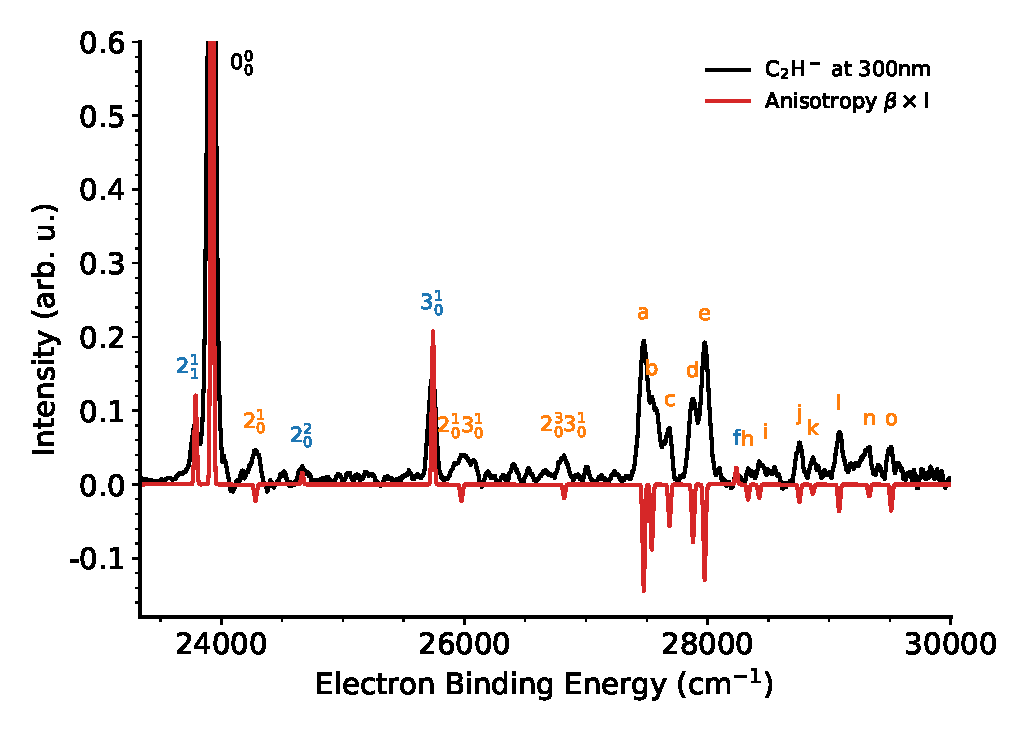
\includegraphics[width=0.6\textwidth]{figures/Fig6}
	\caption{Photoelectron spectrum of C$_2$H$^-$ at 300~nm, compared to anisotropy measurements, presented as $\beta\times I$. For each resolved transition the anisotropy parameter was determined from Eq.~(\ref{eq:10}) and multiplied by the corresponding photoelectron intensity. This allows for the sign $(+/-)$ of each transitions to be readily identified.}
	\label{fig:6}
\end{figure}

This result demonstrates how experimental anisotropies and calculated transition intensities can be combined to help assign and understand vibronically coupled spectra. An approach that is particularly useful in spectral regions where there are a large number of potential vibronic transitions, making definitive assignments based on energetics alone difficult.



\section{Conclusions} 
High-resolution photoelectron images of C$_2$H$^-$ and C$_2$D$^-$ have been recorded at multiple wavelengths between 355~nm and 266~nm, to investigate vibronic coupling effects in the simplest C$_{2n}$H carbon monohydride chain. The interplay of pseudo Jahn-Teller and Renner Teller coupling between the close lying $\tilde{X}^2\Sigma^+$ and $\tilde{A}^2\Pi$ states results in a complex vibronic spectrum near the $\tilde{A}$ state surface, with the electronic origin split over multiple admixed levels. By transforming to a quasidiabatic representation, the effect of these coupling interactions may be accurately simulated. A KDC Hamiltonian was constructed, and parametrized using the high-level EOM-CCSDT quantum chemical approach and the quasidiabatic ansatz. The resulting simulated photoelectron spectra of C$_2$H$^-$ and C$_2$D$^-$ reproduce the experimental data, particularly in the complex energy region of the $\tilde{A}$ state origin. Photoelectron anisotropy parameters were also measured for dominant transitions, at a range of wavelengths. The sign $(+/-)$ of the electron anisotropy parameter, when compared with the calculated vibronic symmetry, allowed even weak or partially resolved transitions to be assigned.

The excellent agreement between the experimental and calculated spectra of this work
demonstrate that electronic spectra, complicated by vibronic coupling effects, may still be accurately simulated by using a quasidiabatic treatment, as parametrized by appropriate quantum chemical methodology. This approach may be applied to larger, less well known, C$_{2n}$H species, which may help guide the search for these molecules in astronomical studies, and help identify potential DIB carriers. It is especially encouraging that the fairly modest parametrization used here works so well for C$_2$H, as this bodes well for its extension to larger systems.


\section*{Supplementary Materials}
See supplementary material for the complete list of C$_2$H and C$_2$D photoelectron transitions and assignments.


\begin{acknowledgments}
	This research was supported by the Australian Research Council Discovery
	Project Grants DP160102585 and DP190103151.  
\end{acknowledgments}

\section*{Data Availability}
The data that support the findings of this study are available from the corresponding author upon reasonable request.

%\bibliography{Laws_C2H}
%merlin.mbs aipnum4-1.bst 2010-07-25 4.21a (PWD, AO, DPC) hacked
%Control: key (0)
%Control: author (8) initials jnrlst
%Control: editor formatted (1) identically to author
%Control: production of article title (0) allowed
%Control: page (1) range
%Control: year (1) truncated
%Control: production of eprint (0) enabled
\begin{thebibliography}{98}%
	\makeatletter
	\providecommand \@ifxundefined [1]{%
		\@ifx{#1\undefined}
	}%
	\providecommand \@ifnum [1]{%
		\ifnum #1\expandafter \@firstoftwo
		\else \expandafter \@secondoftwo
		\fi
	}%
	\providecommand \@ifx [1]{%
		\ifx #1\expandafter \@firstoftwo
		\else \expandafter \@secondoftwo
		\fi
	}%
	\providecommand \natexlab [1]{#1}%
	\providecommand \enquote  [1]{``#1''}%
	\providecommand \bibnamefont  [1]{#1}%
	\providecommand \bibfnamefont [1]{#1}%
	\providecommand \citenamefont [1]{#1}%
	\providecommand \href@noop [0]{\@secondoftwo}%
	\providecommand \href [0]{\begingroup \@sanitize@url \@href}%
	\providecommand \@href[1]{\@@startlink{#1}\@@href}%
	\providecommand \@@href[1]{\endgroup#1\@@endlink}%
	\providecommand \@sanitize@url [0]{\catcode `\\12\catcode `\$12\catcode
		`\&12\catcode `\#12\catcode `\^12\catcode `\_12\catcode `\%12\relax}%
	\providecommand \@@startlink[1]{}%
	\providecommand \@@endlink[0]{}%
	\providecommand \url  [0]{\begingroup\@sanitize@url \@url }%
	\providecommand \@url [1]{\endgroup\@href {#1}{\urlprefix }}%
	\providecommand \urlprefix  [0]{URL }%
	\providecommand \Eprint [0]{\href }%
	\providecommand \doibase [0]{http://dx.doi.org/}%
	\providecommand \selectlanguage [0]{\@gobble}%
	\providecommand \bibinfo  [0]{\@secondoftwo}%
	\providecommand \bibfield  [0]{\@secondoftwo}%
	\providecommand \translation [1]{[#1]}%
	\providecommand \BibitemOpen [0]{}%
	\providecommand \bibitemStop [0]{}%
	\providecommand \bibitemNoStop [0]{.\EOS\space}%
	\providecommand \EOS [0]{\spacefactor3000\relax}%
	\providecommand \BibitemShut  [1]{\csname bibitem#1\endcsname}%
	\let\auto@bib@innerbib\@empty
	%</preamble>
	\bibitem [{\citenamefont {Kiefer}, \citenamefont {Von~Drasek},\ and\
		\citenamefont {Von~Drasek}(1990)}]{kie90}%
	\BibitemOpen
	\bibfield  {author} {\bibinfo {author} {\bibfnamefont {J.~H.}\ \bibnamefont
			{Kiefer}}, \bibinfo {author} {\bibfnamefont {W.~A.}\ \bibnamefont
			{Von~Drasek}}, \ and\ \bibinfo {author} {\bibfnamefont {W.~A.}\ \bibnamefont
			{Von~Drasek}},\ }\bibfield  {title} {\enquote {\bibinfo {title} {The
				mechanism of the homogeneous pyrolysis of acetylene},}\ }\href {\doibase
		https://doi.org/10.1002/kin.550220710} {\bibfield  {journal} {\bibinfo
			{journal} {International Journal of Chemical Kinetics}\ }\textbf {\bibinfo
			{volume} {22}},\ \bibinfo {pages} {747--786} (\bibinfo {year}
		{1990})}\BibitemShut {NoStop}%
	\bibitem [{\citenamefont {Kiefer}\ \emph {et~al.}(1992)\citenamefont {Kiefer},
		\citenamefont {Sidhu}, \citenamefont {Kern}, \citenamefont {Xie},
		\citenamefont {Chen},\ and\ \citenamefont {Harding}}]{kie92}%
	\BibitemOpen
	\bibfield  {author} {\bibinfo {author} {\bibfnamefont {J.~H.}\ \bibnamefont
			{Kiefer}}, \bibinfo {author} {\bibfnamefont {S.~S.}\ \bibnamefont {Sidhu}},
		\bibinfo {author} {\bibfnamefont {R.~D.}\ \bibnamefont {Kern}}, \bibinfo
		{author} {\bibfnamefont {K.}~\bibnamefont {Xie}}, \bibinfo {author}
		{\bibfnamefont {H.}~\bibnamefont {Chen}}, \ and\ \bibinfo {author}
		{\bibfnamefont {L.~B.}\ \bibnamefont {Harding}},\ }\bibfield  {title}
	{\enquote {\bibinfo {title} {The homogeneous pyrolysis of acetylene ii: The
				high temperature radical chain mechanism},}\ }\href {\doibase
		10.1080/00102209208951815} {\bibfield  {journal} {\bibinfo  {journal}
			{Combustion Science and Technology}\ }\textbf {\bibinfo {volume} {82}},\
		\bibinfo {pages} {101--130} (\bibinfo {year} {1992})}\BibitemShut {NoStop}%
	\bibitem [{\citenamefont {Boullart}\ \emph {et~al.}(1996)\citenamefont
		{Boullart}, \citenamefont {Devriendt}, \citenamefont {Borms},\ and\
		\citenamefont {Peeters}}]{bou96}%
	\BibitemOpen
	\bibfield  {author} {\bibinfo {author} {\bibfnamefont {W.}~\bibnamefont
			{Boullart}}, \bibinfo {author} {\bibfnamefont {K.}~\bibnamefont {Devriendt}},
		\bibinfo {author} {\bibfnamefont {R.}~\bibnamefont {Borms}}, \ and\ \bibinfo
		{author} {\bibfnamefont {J.}~\bibnamefont {Peeters}},\ }\bibfield  {title}
	{\enquote {\bibinfo {title} {{Identification of the Sequence CH($^2\Pi$) +
					C$_2$H$_2$ $\rightarrow$ C$_3$H$_2$ + H (and C$_3$H + H$_2$) Followed by
					C$_3$H$_2$ + O $\rightarrow$ C$_2$H + HCO (or H + CO) as C$_2$H Source in
					C$_2$H$_2$/O/H Atomic Flames}},}\ }\href {\doibase 10.1021/jp951995o}
	{\bibfield  {journal} {\bibinfo  {journal} {The Journal of Physical
				Chemistry}\ }\textbf {\bibinfo {volume} {100}},\ \bibinfo {pages} {998--1007}
		(\bibinfo {year} {1996})}\BibitemShut {NoStop}%
	\bibitem [{\citenamefont {Irvine}, \citenamefont {Ohishi},\ and\ \citenamefont
		{Kaifu}(1991)}]{wil91}%
	\BibitemOpen
	\bibfield  {author} {\bibinfo {author} {\bibfnamefont {W.~M.}\ \bibnamefont
			{Irvine}}, \bibinfo {author} {\bibfnamefont {M.}~\bibnamefont {Ohishi}}, \
		and\ \bibinfo {author} {\bibfnamefont {N.}~\bibnamefont {Kaifu}},\ }\bibfield
	{title} {\enquote {\bibinfo {title} {Chemical abundances in cold, dark
				interstellar clouds},}\ }\href {\doibase
		https://doi.org/10.1016/0019-1035(91)90120-I} {\bibfield  {journal} {\bibinfo
			{journal} {Icarus}\ }\textbf {\bibinfo {volume} {91}},\ \bibinfo {pages}
		{2--6} (\bibinfo {year} {1991})}\BibitemShut {NoStop}%
	\bibitem [{\citenamefont {Vuitton}\ \emph {et~al.}(2001)\citenamefont
		{Vuitton}, \citenamefont {Scemama}, \citenamefont {Gazeau}, \citenamefont
		{Chaquin},\ and\ \citenamefont {B\'{e}nilan}}]{vui01}%
	\BibitemOpen
	\bibfield  {author} {\bibinfo {author} {\bibfnamefont {V.}~\bibnamefont
			{Vuitton}}, \bibinfo {author} {\bibfnamefont {A.}~\bibnamefont {Scemama}},
		\bibinfo {author} {\bibfnamefont {M.-C.}\ \bibnamefont {Gazeau}}, \bibinfo
		{author} {\bibfnamefont {P.}~\bibnamefont {Chaquin}}, \ and\ \bibinfo
		{author} {\bibfnamefont {Y.}~\bibnamefont {B\'{e}nilan}},\ }\bibfield
	{title} {\enquote {\bibinfo {title} {{IR and UV spectroscopic data for
					polyynes: Predictions for long carbon chain compounds in Titan's
					atmosphere}},}\ }\href {\doibase
		https://doi.org/10.1016/S0273-1177(01)00059-X} {\bibfield  {journal}
		{\bibinfo  {journal} {Advances in Space Research}\ }\textbf {\bibinfo
			{volume} {27}},\ \bibinfo {pages} {283--288} (\bibinfo {year}
		{2001})}\BibitemShut {NoStop}%
	\bibitem [{\citenamefont {Wilson}\ and\ \citenamefont {Atreya}(2003)}]{wil03}%
	\BibitemOpen
	\bibfield  {author} {\bibinfo {author} {\bibfnamefont {E.}~\bibnamefont
			{Wilson}}\ and\ \bibinfo {author} {\bibfnamefont {S.}~\bibnamefont
			{Atreya}},\ }\bibfield  {title} {\enquote {\bibinfo {title} {Chemical sources
				of haze formation in {Titan's} atmosphere},}\ }\href {\doibase
		https://doi.org/10.1016/j.pss.2003.06.003} {\bibfield  {journal} {\bibinfo
			{journal} {Planetary and Space Science}\ }\textbf {\bibinfo {volume} {51}},\
		\bibinfo {pages} {1017--1033} (\bibinfo {year} {2003})},\ \bibinfo {note}
	{surfaces and Atmospheres of the Outer Planets their Satellites and Ring
		Systems}\BibitemShut {NoStop}%
	\bibitem [{\citenamefont {Dobrijevic}\ \emph {et~al.}(2016)\citenamefont
		{Dobrijevic}, \citenamefont {Loison}, \citenamefont {Hickson},\ and\
		\citenamefont {Gronoff}}]{dob16}%
	\BibitemOpen
	\bibfield  {author} {\bibinfo {author} {\bibfnamefont {M.}~\bibnamefont
			{Dobrijevic}}, \bibinfo {author} {\bibfnamefont {J.}~\bibnamefont {Loison}},
		\bibinfo {author} {\bibfnamefont {K.}~\bibnamefont {Hickson}}, \ and\
		\bibinfo {author} {\bibfnamefont {G.}~\bibnamefont {Gronoff}},\ }\bibfield
	{title} {\enquote {\bibinfo {title} {{1D}-coupled photochemical model of
				neutrals, cations and anions in the atmosphere of {Titan}},}\ }\href
	{\doibase https://doi.org/10.1016/j.icarus.2015.12.045} {\bibfield  {journal}
		{\bibinfo  {journal} {Icarus}\ }\textbf {\bibinfo {volume} {268}},\ \bibinfo
		{pages} {313 -- 339} (\bibinfo {year} {2016})}\BibitemShut {NoStop}%
	\bibitem [{\citenamefont {Jackson}\ \emph {et~al.}(1996)\citenamefont
		{Jackson}, \citenamefont {Blunt}, \citenamefont {Lin}, \citenamefont {Green},
		\citenamefont {Olivera}, \citenamefont {Fink}, \citenamefont {Bao},
		\citenamefont {Urdahl}, \citenamefont {Mohammad},\ and\ \citenamefont
		{Zahedi}}]{jac96}%
	\BibitemOpen
	\bibfield  {author} {\bibinfo {author} {\bibfnamefont {W.~M.}\ \bibnamefont
			{Jackson}}, \bibinfo {author} {\bibfnamefont {V.}~\bibnamefont {Blunt}},
		\bibinfo {author} {\bibfnamefont {H.}~\bibnamefont {Lin}}, \bibinfo {author}
		{\bibfnamefont {M.}~\bibnamefont {Green}}, \bibinfo {author} {\bibfnamefont
			{G.}~\bibnamefont {Olivera}}, \bibinfo {author} {\bibfnamefont {W.~H.}\
			\bibnamefont {Fink}}, \bibinfo {author} {\bibfnamefont {Y.}~\bibnamefont
			{Bao}}, \bibinfo {author} {\bibfnamefont {R.~S.}\ \bibnamefont {Urdahl}},
		\bibinfo {author} {\bibfnamefont {F.}~\bibnamefont {Mohammad}}, \ and\
		\bibinfo {author} {\bibfnamefont {M.}~\bibnamefont {Zahedi}},\ }\bibfield
	{title} {\enquote {\bibinfo {title} {Non-adiabatic interactions in excited
				{C$_2$H} molecules and their relationship to {C$_2$} formation in comets},}\
	}\href {\doibase 10.1007/BF00644319} {\bibfield  {journal} {\bibinfo
			{journal} {Astrophysics and Space Science}\ }\textbf {\bibinfo {volume}
			{236}},\ \bibinfo {pages} {29--47} (\bibinfo {year} {1996})}\BibitemShut
	{NoStop}%
	\bibitem [{\citenamefont {{Ziurys}}\ \emph {et~al.}(1982)\citenamefont
		{{Ziurys}}, \citenamefont {{Saykally}}, \citenamefont {{Plambeck}},\ and\
		\citenamefont {{Erickson}}}]{ziu82}%
	\BibitemOpen
	\bibfield  {author} {\bibinfo {author} {\bibfnamefont {L.~M.}\ \bibnamefont
			{{Ziurys}}}, \bibinfo {author} {\bibfnamefont {R.~J.}\ \bibnamefont
			{{Saykally}}}, \bibinfo {author} {\bibfnamefont {R.~L.}\ \bibnamefont
			{{Plambeck}}}, \ and\ \bibinfo {author} {\bibfnamefont {N.~R.}\ \bibnamefont
			{{Erickson}}},\ }\bibfield  {title} {\enquote {\bibinfo {title} {{Detection
					of the N=3-2 transition of CCH in Orion and determination of the molecular
					rotational constants}},}\ }\href {\doibase 10.1086/159709} {\bibfield
		{journal} {\bibinfo  {journal} {The Astrophysical Journal}\ }\textbf
		{\bibinfo {volume} {254}},\ \bibinfo {pages} {94--99} (\bibinfo {year}
		{1982})}\BibitemShut {NoStop}%
	\bibitem [{\citenamefont {Gupta}\ \emph {et~al.}(2009)\citenamefont {Gupta},
		\citenamefont {Gottlieb}, \citenamefont {McCarthy},\ and\ \citenamefont
		{Thaddeus}}]{gup09}%
	\BibitemOpen
	\bibfield  {author} {\bibinfo {author} {\bibfnamefont {H.}~\bibnamefont
			{Gupta}}, \bibinfo {author} {\bibfnamefont {C.~A.}\ \bibnamefont {Gottlieb}},
		\bibinfo {author} {\bibfnamefont {M.~C.}\ \bibnamefont {McCarthy}}, \ and\
		\bibinfo {author} {\bibfnamefont {P.}~\bibnamefont {Thaddeus}},\ }\bibfield
	{title} {\enquote {\bibinfo {title} {A survey of {C$_4$H, C$_6$H, and
					C$_6$H$^-$ with the Green Bank Telescope}},}\ }\href {\doibase
		10.1088/0004-637x/691/2/1494} {\bibfield  {journal} {\bibinfo  {journal} {The
				Astrophysical Journal}\ }\textbf {\bibinfo {volume} {691}},\ \bibinfo {pages}
		{1494--1500} (\bibinfo {year} {2009})}\BibitemShut {NoStop}%
	\bibitem [{\citenamefont {Beuther}\ \emph {et~al.}(2008)\citenamefont
		{Beuther}, \citenamefont {Semenov}, \citenamefont {Henning},\ and\
		\citenamefont {Linz}}]{beu08}%
	\BibitemOpen
	\bibfield  {author} {\bibinfo {author} {\bibfnamefont {H.}~\bibnamefont
			{Beuther}}, \bibinfo {author} {\bibfnamefont {D.}~\bibnamefont {Semenov}},
		\bibinfo {author} {\bibfnamefont {T.}~\bibnamefont {Henning}}, \ and\
		\bibinfo {author} {\bibfnamefont {H.}~\bibnamefont {Linz}},\ }\bibfield
	{title} {\enquote {\bibinfo {title} {Ethynyl ({C$_2$H}) in massive star
				formation: Tracing the initial conditions?}}\ }\href
	{http://stacks.iop.org/1538-4357/675/i=1/a=L33} {\bibfield  {journal}
		{\bibinfo  {journal} {The Astrophysical Journal Letters}\ }\textbf {\bibinfo
			{volume} {675}},\ \bibinfo {pages} {L33} (\bibinfo {year}
		{2008})}\BibitemShut {NoStop}%
	\bibitem [{\citenamefont {Jiang}\ \emph {et~al.}(2015)\citenamefont {Jiang},
		\citenamefont {Liu}, \citenamefont {Zhang}, \citenamefont {Wang},
		\citenamefont {Zhang}, \citenamefont {Li}, \citenamefont {Gao},\ and\
		\citenamefont {Gu}}]{jia15}%
	\BibitemOpen
	\bibfield  {author} {\bibinfo {author} {\bibfnamefont {X.-J.}\ \bibnamefont
			{Jiang}}, \bibinfo {author} {\bibfnamefont {H.~B.}\ \bibnamefont {Liu}},
		\bibinfo {author} {\bibfnamefont {Q.}~\bibnamefont {Zhang}}, \bibinfo
		{author} {\bibfnamefont {J.}~\bibnamefont {Wang}}, \bibinfo {author}
		{\bibfnamefont {Z.-Y.}\ \bibnamefont {Zhang}}, \bibinfo {author}
		{\bibfnamefont {J.}~\bibnamefont {Li}}, \bibinfo {author} {\bibfnamefont
			{Y.}~\bibnamefont {Gao}}, \ and\ \bibinfo {author} {\bibfnamefont
			{Q.}~\bibnamefont {Gu}},\ }\bibfield  {title} {\enquote {\bibinfo {title}
			{{{SMA} Observations of C$_2$H in High-Mass Star-Forming Regions}},}\ }\href
	{\doibase 10.1088/0004-637x/808/2/114} {\bibfield  {journal} {\bibinfo
			{journal} {The Astrophysical Journal}\ }\textbf {\bibinfo {volume} {808}},\
		\bibinfo {pages} {114} (\bibinfo {year} {2015})}\BibitemShut {NoStop}%
	\bibitem [{\citenamefont {Douglas}(1977)}]{dou77}%
	\BibitemOpen
	\bibfield  {author} {\bibinfo {author} {\bibfnamefont {A.}~\bibnamefont
			{Douglas}},\ }\bibfield  {title} {\enquote {\bibinfo {title} {Origin of
				diffuse interstellar lines},}\ }\href
	{https://www.nature.com/articles/269130a0} {\bibfield  {journal} {\bibinfo
			{journal} {Nature}\ }\textbf {\bibinfo {volume} {269}},\ \bibinfo {pages}
		{130--132} (\bibinfo {year} {1977})}\BibitemShut {NoStop}%
	\bibitem [{\citenamefont {Fulara}\ \emph {et~al.}(1993)\citenamefont {Fulara},
		\citenamefont {Lessen}, \citenamefont {Freivogel},\ and\ \citenamefont
		{Maier}}]{ful93}%
	\BibitemOpen
	\bibfield  {author} {\bibinfo {author} {\bibfnamefont {J.}~\bibnamefont
			{Fulara}}, \bibinfo {author} {\bibfnamefont {D.}~\bibnamefont {Lessen}},
		\bibinfo {author} {\bibfnamefont {P.}~\bibnamefont {Freivogel}}, \ and\
		\bibinfo {author} {\bibfnamefont {P.}~\bibnamefont {Maier}},\ }\bibfield
	{title} {\enquote {\bibinfo {title} {Laboratory evidence for highly
				unsaturated hydrocarbons as carriers of some of the diffuse interstellar
				bands},}\ }\href {https://www.nature.com/articles/366439a0} {\bibfield
		{journal} {\bibinfo  {journal} {Nature}\ }\textbf {\bibinfo {volume} {366}},\
		\bibinfo {pages} {439--441} (\bibinfo {year} {1993})}\BibitemShut {NoStop}%
	\bibitem [{\citenamefont {{Watson}}(1994)}]{wat94}%
	\BibitemOpen
	\bibfield  {author} {\bibinfo {author} {\bibfnamefont {J.~K.}\ \bibnamefont
			{{Watson}}},\ }\bibfield  {title} {\enquote {\bibinfo {title} {{Homologous
					Series of Diffuse Interstellar Bands}},}\ }\href {\doibase 10.1086/175030}
	{\bibfield  {journal} {\bibinfo  {journal} {The Astrophysical Journal}\
		}\textbf {\bibinfo {volume} {437}},\ \bibinfo {pages} {678} (\bibinfo {year}
		{1994})}\BibitemShut {NoStop}%
	\bibitem [{\citenamefont {Fulara}\ and\ \citenamefont
		{Krelowski}(2000)}]{ful00}%
	\BibitemOpen
	\bibfield  {author} {\bibinfo {author} {\bibfnamefont {J.}~\bibnamefont
			{Fulara}}\ and\ \bibinfo {author} {\bibfnamefont {J.}~\bibnamefont
			{Krelowski}},\ }\bibfield  {title} {\enquote {\bibinfo {title} {Origin of
				diffuse interstellar bands: spectroscopic studies of their possible
				carriers},}\ }\href {\doibase https://doi.org/10.1016/S1387-6473(00)00108-1}
	{\bibfield  {journal} {\bibinfo  {journal} {New Astronomy Reviews}\ }\textbf
		{\bibinfo {volume} {44}},\ \bibinfo {pages} {581--597} (\bibinfo {year}
		{2000})}\BibitemShut {NoStop}%
	\bibitem [{\citenamefont {Schmidt Timothy~W.}(2005)}]{sch05}%
	\BibitemOpen
	\bibfield  {author} {\bibinfo {author} {\bibfnamefont {S.~R.~G.}\
			\bibnamefont {Schmidt Timothy~W.}},\ }\bibfield  {title} {\enquote {\bibinfo
			{title} {The optical spectroscopy of extraterrestrial molecules.}}\ }\href
	{https://www.publish.csiro.au/ch/Fulltext/CH04269#R14} {\bibfield  {journal}
		{\bibinfo  {journal} {Australian Journal of Chemistry}\ }\textbf {\bibinfo
			{volume} {58}},\ \bibinfo {pages} {69--81} (\bibinfo {year}
		{2005})}\BibitemShut {NoStop}%
	\bibitem [{\citenamefont {Millar}, \citenamefont {Walsh},\ and\ \citenamefont
		{Field}(2017)}]{mil17}%
	\BibitemOpen
	\bibfield  {author} {\bibinfo {author} {\bibfnamefont {T.~J.}\ \bibnamefont
			{Millar}}, \bibinfo {author} {\bibfnamefont {C.}~\bibnamefont {Walsh}}, \
		and\ \bibinfo {author} {\bibfnamefont {T.~A.}\ \bibnamefont {Field}},\
	}\bibfield  {title} {\enquote {\bibinfo {title} {Negative ions in space},}\
	}\href {\doibase 10.1021/acs.chemrev.6b00480} {\bibfield  {journal} {\bibinfo
			{journal} {Chemical Reviews}\ }\textbf {\bibinfo {volume} {117}},\ \bibinfo
		{pages} {1765--1795} (\bibinfo {year} {2017})},\ \bibinfo {note} {pMID:
		28112897}\BibitemShut {NoStop}%
	\bibitem [{\citenamefont {McCarthy}\ \emph {et~al.}(2006)\citenamefont
		{McCarthy}, \citenamefont {Gottlieb}, \citenamefont {Gupta},\ and\
		\citenamefont {Thaddeus}}]{mcc06}%
	\BibitemOpen
	\bibfield  {author} {\bibinfo {author} {\bibfnamefont {M.~C.}\ \bibnamefont
			{McCarthy}}, \bibinfo {author} {\bibfnamefont {C.~A.}\ \bibnamefont
			{Gottlieb}}, \bibinfo {author} {\bibfnamefont {H.}~\bibnamefont {Gupta}}, \
		and\ \bibinfo {author} {\bibfnamefont {P.}~\bibnamefont {Thaddeus}},\
	}\bibfield  {title} {\enquote {\bibinfo {title} {{Laboratory and Astronomical
					Identification of the Negative Molecular Ion C$_6$H$^-$}},}\ }\href {\doibase
		10.1086/510238} {\bibfield  {journal} {\bibinfo  {journal} {The Astrophysical
				Journal}\ }\textbf {\bibinfo {volume} {652}},\ \bibinfo {pages} {L141--L144}
		(\bibinfo {year} {2006})}\BibitemShut {NoStop}%
	\bibitem [{\citenamefont {Cernicharo}\ \emph {et~al.}(2007)\citenamefont
		{Cernicharo}, \citenamefont {Gu\'elin}, \citenamefont {Ag\'undez},
		\citenamefont {Kawaguchi}, \citenamefont {McCarthy},\ and\ \citenamefont
		{Thaddeus}}]{cer07}%
	\BibitemOpen
	\bibfield  {author} {\bibinfo {author} {\bibfnamefont {J.}~\bibnamefont
			{Cernicharo}}, \bibinfo {author} {\bibfnamefont {M.}~\bibnamefont
			{Gu\'elin}}, \bibinfo {author} {\bibfnamefont {M.}~\bibnamefont {Ag\'undez}},
		\bibinfo {author} {\bibfnamefont {K.}~\bibnamefont {Kawaguchi}}, \bibinfo
		{author} {\bibfnamefont {M.}~\bibnamefont {McCarthy}}, \ and\ \bibinfo
		{author} {\bibfnamefont {P.}~\bibnamefont {Thaddeus}},\ }\bibfield  {title}
	{\enquote {\bibinfo {title} {{Astronomical detection of C$_4$H$^-$, the
					second interstellar anion*}},}\ }\href {\doibase 10.1051/0004-6361:20077415}
	{\bibfield  {journal} {\bibinfo  {journal} {Astronomy \& Astropysics}\
		}\textbf {\bibinfo {volume} {467}},\ \bibinfo {pages} {L37--L40} (\bibinfo
		{year} {2007})}\BibitemShut {NoStop}%
	\bibitem [{\citenamefont {Br\"{u}nken}\ \emph {et~al.}(2007)\citenamefont
		{Br\"{u}nken}, \citenamefont {Gupta}, \citenamefont {Gottlieb}, \citenamefont
		{McCarthy},\ and\ \citenamefont {Thaddeus}}]{bru07}%
	\BibitemOpen
	\bibfield  {author} {\bibinfo {author} {\bibfnamefont {S.}~\bibnamefont
			{Br\"{u}nken}}, \bibinfo {author} {\bibfnamefont {H.}~\bibnamefont {Gupta}},
		\bibinfo {author} {\bibfnamefont {C.~A.}\ \bibnamefont {Gottlieb}}, \bibinfo
		{author} {\bibfnamefont {M.~C.}\ \bibnamefont {McCarthy}}, \ and\ \bibinfo
		{author} {\bibfnamefont {P.}~\bibnamefont {Thaddeus}},\ }\bibfield  {title}
	{\enquote {\bibinfo {title} {{Detection of the Carbon Chain Negative Ion
					C$_8$H$^-$ in {TMC}-1}},}\ }\href {\doibase 10.1086/520703} {\bibfield
		{journal} {\bibinfo  {journal} {The Astrophysical Journal}\ }\textbf
		{\bibinfo {volume} {664}},\ \bibinfo {pages} {L43--L46} (\bibinfo {year}
		{2007})}\BibitemShut {NoStop}%
	\bibitem [{\citenamefont {Remijan}\ \emph {et~al.}(2007)\citenamefont
		{Remijan}, \citenamefont {Hollis}, \citenamefont {Lovas}, \citenamefont
		{Cordiner}, \citenamefont {Millar}, \citenamefont {Markwick-Kemper},\ and\
		\citenamefont {Jewell}}]{rem07}%
	\BibitemOpen
	\bibfield  {author} {\bibinfo {author} {\bibfnamefont {A.~J.}\ \bibnamefont
			{Remijan}}, \bibinfo {author} {\bibfnamefont {J.~M.}\ \bibnamefont {Hollis}},
		\bibinfo {author} {\bibfnamefont {F.~J.}\ \bibnamefont {Lovas}}, \bibinfo
		{author} {\bibfnamefont {M.~A.}\ \bibnamefont {Cordiner}}, \bibinfo {author}
		{\bibfnamefont {T.~J.}\ \bibnamefont {Millar}}, \bibinfo {author}
		{\bibfnamefont {A.~J.}\ \bibnamefont {Markwick-Kemper}}, \ and\ \bibinfo
		{author} {\bibfnamefont {P.~R.}\ \bibnamefont {Jewell}},\ }\bibfield  {title}
	{\enquote {\bibinfo {title} {{Detection of C$_8$H$^-$ and Comparison with
					C$_8$H toward {IRC} $+$10 216}},}\ }\href {\doibase 10.1086/520704}
	{\bibfield  {journal} {\bibinfo  {journal} {The Astrophysical Journal}\
		}\textbf {\bibinfo {volume} {664}},\ \bibinfo {pages} {L47--L50} (\bibinfo
		{year} {2007})}\BibitemShut {NoStop}%
	\bibitem [{\citenamefont {Cordiner}\ \emph {et~al.}(2013)\citenamefont
		{Cordiner}, \citenamefont {Buckle}, \citenamefont {Wirstr\"{o}m},
		\citenamefont {Olofsson},\ and\ \citenamefont {Charnley}}]{cor13}%
	\BibitemOpen
	\bibfield  {author} {\bibinfo {author} {\bibfnamefont {M.~A.}\ \bibnamefont
			{Cordiner}}, \bibinfo {author} {\bibfnamefont {J.~V.}\ \bibnamefont
			{Buckle}}, \bibinfo {author} {\bibfnamefont {E.~S.}\ \bibnamefont
			{Wirstr\"{o}m}}, \bibinfo {author} {\bibfnamefont {A.~O.~H.}\ \bibnamefont
			{Olofsson}}, \ and\ \bibinfo {author} {\bibfnamefont {S.~B.}\ \bibnamefont
			{Charnley}},\ }\bibfield  {title} {\enquote {\bibinfo {title} {{On the
					Ubiquity of Molecular Anions in the Dense Interstellar Medium}},}\ }\href
	{\doibase 10.1088/0004-637x/770/1/48} {\bibfield  {journal} {\bibinfo
			{journal} {The Astrophysical Journal}\ }\textbf {\bibinfo {volume} {770}},\
		\bibinfo {pages} {48} (\bibinfo {year} {2013})}\BibitemShut {NoStop}%
	\bibitem [{\citenamefont {Sakai}\ \emph {et~al.}(2010)\citenamefont {Sakai},
		\citenamefont {Shiino}, \citenamefont {Hirota}, \citenamefont {Sakai},\ and\
		\citenamefont {Yamamoto}}]{sak10}%
	\BibitemOpen
	\bibfield  {author} {\bibinfo {author} {\bibfnamefont {N.}~\bibnamefont
			{Sakai}}, \bibinfo {author} {\bibfnamefont {T.}~\bibnamefont {Shiino}},
		\bibinfo {author} {\bibfnamefont {T.}~\bibnamefont {Hirota}}, \bibinfo
		{author} {\bibfnamefont {T.}~\bibnamefont {Sakai}}, \ and\ \bibinfo {author}
		{\bibfnamefont {S.}~\bibnamefont {Yamamoto}},\ }\bibfield  {title} {\enquote
		{\bibinfo {title} {{Long Carbon-Chain Molecules and their Anions in the
					Starless Core LUPUS-1A}},}\ }\href {\doibase 10.1088/2041-8205/718/2/l49}
	{\bibfield  {journal} {\bibinfo  {journal} {The Astrophysical Journal}\
		}\textbf {\bibinfo {volume} {718}},\ \bibinfo {pages} {L49--L52} (\bibinfo
		{year} {2010})}\BibitemShut {NoStop}%
	\bibitem [{\citenamefont {Sakai}, \citenamefont {Sakai},\ and\ \citenamefont
		{Yamamoto}(2007)}]{sak07}%
	\BibitemOpen
	\bibfield  {author} {\bibinfo {author} {\bibfnamefont {N.}~\bibnamefont
			{Sakai}}, \bibinfo {author} {\bibfnamefont {T.}~\bibnamefont {Sakai}}, \ and\
		\bibinfo {author} {\bibfnamefont {S.}~\bibnamefont {Yamamoto}},\ }\bibfield
	{title} {\enquote {\bibinfo {title} {Tentative detection of {C$_4$H$^-$
					toward the Low-Mass Protostar {IRAS} 04368$+$2557 in L1527}},}\ }\href
	{\doibase 10.1086/527376} {\bibfield  {journal} {\bibinfo  {journal} {The
				Astrophysical Journal}\ }\textbf {\bibinfo {volume} {673}},\ \bibinfo {pages}
		{L71--L74} (\bibinfo {year} {2007})}\BibitemShut {NoStop}%
	\bibitem [{\citenamefont {Herbst}\ and\ \citenamefont {Osamura}(2008)}]{her08}%
	\BibitemOpen
	\bibfield  {author} {\bibinfo {author} {\bibfnamefont {E.}~\bibnamefont
			{Herbst}}\ and\ \bibinfo {author} {\bibfnamefont {Y.}~\bibnamefont
			{Osamura}},\ }\bibfield  {title} {\enquote {\bibinfo {title} {Calculations on
				the formation rates and mechanisms for {CnH} anions in interstellar and
				circumstellar media},}\ }\href {\doibase 10.1086/587803} {\bibfield
		{journal} {\bibinfo  {journal} {The Astrophysical Journal}\ }\textbf
		{\bibinfo {volume} {679}},\ \bibinfo {pages} {1670--1679} (\bibinfo {year}
		{2008})}\BibitemShut {NoStop}%
	\bibitem [{\citenamefont {Bastian}\ \emph {et~al.}(2019)\citenamefont
		{Bastian}, \citenamefont {Michaelsen}, \citenamefont {Meyer},\ and\
		\citenamefont {Wester}}]{bas19}%
	\BibitemOpen
	\bibfield  {author} {\bibinfo {author} {\bibfnamefont {B.}~\bibnamefont
			{Bastian}}, \bibinfo {author} {\bibfnamefont {T.}~\bibnamefont {Michaelsen}},
		\bibinfo {author} {\bibfnamefont {J.}~\bibnamefont {Meyer}}, \ and\ \bibinfo
		{author} {\bibfnamefont {R.}~\bibnamefont {Wester}},\ }\bibfield  {title}
	{\enquote {\bibinfo {title} {{Anionic Carbon Chain Growth in Reactions of
					C$_2^-$, C$_4^-$, C$_6^-$, C$_2$H$^-$, C$_4$H$^-$, and C$_6$H$^-$ with
					C$_2$H$_2$}},}\ }\href {\doibase 10.3847/1538-4357/ab2042} {\bibfield
		{journal} {\bibinfo  {journal} {The Astrophysical Journal}\ }\textbf
		{\bibinfo {volume} {878}},\ \bibinfo {pages} {162} (\bibinfo {year}
		{2019})}\BibitemShut {NoStop}%
	\bibitem [{\citenamefont {Vuitton}\ \emph {et~al.}(2009)\citenamefont
		{Vuitton}, \citenamefont {Lavvas}, \citenamefont {Yelle}, \citenamefont
		{Galand}, \citenamefont {Wellbrock}, \citenamefont {Lewis}, \citenamefont
		{Coates},\ and\ \citenamefont {Wahlund}}]{vui09}%
	\BibitemOpen
	\bibfield  {author} {\bibinfo {author} {\bibfnamefont {V.}~\bibnamefont
			{Vuitton}}, \bibinfo {author} {\bibfnamefont {P.}~\bibnamefont {Lavvas}},
		\bibinfo {author} {\bibfnamefont {R.}~\bibnamefont {Yelle}}, \bibinfo
		{author} {\bibfnamefont {M.}~\bibnamefont {Galand}}, \bibinfo {author}
		{\bibfnamefont {A.}~\bibnamefont {Wellbrock}}, \bibinfo {author}
		{\bibfnamefont {G.}~\bibnamefont {Lewis}}, \bibinfo {author} {\bibfnamefont
			{A.}~\bibnamefont {Coates}}, \ and\ \bibinfo {author} {\bibfnamefont {J.-E.}\
			\bibnamefont {Wahlund}},\ }\bibfield  {title} {\enquote {\bibinfo {title}
			{{Negative ion chemistry in Titan's upper atmosphere}},}\ }\href {\doibase
		https://doi.org/10.1016/j.pss.2009.04.004} {\bibfield  {journal} {\bibinfo
			{journal} {Planetary and Space Science}\ }\textbf {\bibinfo {volume} {57}},\
		\bibinfo {pages} {1558--1572} (\bibinfo {year} {2009})},\ \bibinfo {note}
	{surfaces and Atmospheres of the Outer Planets, Their Satellites and Ring
		Systems: Part V}\BibitemShut {NoStop}%
	\bibitem [{\citenamefont {Desai}\ \emph {et~al.}(2017)\citenamefont {Desai},
		\citenamefont {Coates}, \citenamefont {Wellbrock}, \citenamefont {Vuitton},
		\citenamefont {Crary}, \citenamefont {Gonz{\'{a}}lez-Caniulef}, \citenamefont
		{Shebanits}, \citenamefont {Jones}, \citenamefont {Lewis}, \citenamefont
		{Waite}, \citenamefont {Cordiner}, \citenamefont {Taylor}, \citenamefont
		{Kataria}, \citenamefont {Wahlund}, \citenamefont {Edberg},\ and\
		\citenamefont {Sittler}}]{des17}%
	\BibitemOpen
	\bibfield  {author} {\bibinfo {author} {\bibfnamefont {R.~T.}\ \bibnamefont
			{Desai}}, \bibinfo {author} {\bibfnamefont {A.~J.}\ \bibnamefont {Coates}},
		\bibinfo {author} {\bibfnamefont {A.}~\bibnamefont {Wellbrock}}, \bibinfo
		{author} {\bibfnamefont {V.}~\bibnamefont {Vuitton}}, \bibinfo {author}
		{\bibfnamefont {F.~J.}\ \bibnamefont {Crary}}, \bibinfo {author}
		{\bibfnamefont {D.}~\bibnamefont {Gonz{\'{a}}lez-Caniulef}}, \bibinfo
		{author} {\bibfnamefont {O.}~\bibnamefont {Shebanits}}, \bibinfo {author}
		{\bibfnamefont {G.~H.}\ \bibnamefont {Jones}}, \bibinfo {author}
		{\bibfnamefont {G.~R.}\ \bibnamefont {Lewis}}, \bibinfo {author}
		{\bibfnamefont {J.~H.}\ \bibnamefont {Waite}}, \bibinfo {author}
		{\bibfnamefont {M.}~\bibnamefont {Cordiner}}, \bibinfo {author}
		{\bibfnamefont {S.~A.}\ \bibnamefont {Taylor}}, \bibinfo {author}
		{\bibfnamefont {D.~O.}\ \bibnamefont {Kataria}}, \bibinfo {author}
		{\bibfnamefont {J.-E.}\ \bibnamefont {Wahlund}}, \bibinfo {author}
		{\bibfnamefont {N.~J.~T.}\ \bibnamefont {Edberg}}, \ and\ \bibinfo {author}
		{\bibfnamefont {E.~C.}\ \bibnamefont {Sittler}},\ }\bibfield  {title}
	{\enquote {\bibinfo {title} {Carbon chain anions and the growth of complex
				organic molecules in titan's ionosphere},}\ }\href {\doibase
		10.3847/2041-8213/aa7851} {\bibfield  {journal} {\bibinfo  {journal} {The
				Astrophysical Journal}\ }\textbf {\bibinfo {volume} {844}},\ \bibinfo {pages}
		{L18} (\bibinfo {year} {2017})}\BibitemShut {NoStop}%
	\bibitem [{\citenamefont {Mukundan}\ and\ \citenamefont
		{Bhardwaj}(2018)}]{vri18}%
	\BibitemOpen
	\bibfield  {author} {\bibinfo {author} {\bibfnamefont {V.}~\bibnamefont
			{Mukundan}}\ and\ \bibinfo {author} {\bibfnamefont {A.}~\bibnamefont
			{Bhardwaj}},\ }\bibfield  {title} {\enquote {\bibinfo {title} {A model for
				negative ion chemistry in {Titan's} ionosphere},}\ }\href {\doibase
		10.3847/1538-4357/aab1f5} {\bibfield  {journal} {\bibinfo  {journal} {The
				Astrophysical Journal}\ }\textbf {\bibinfo {volume} {856}},\ \bibinfo {pages}
		{168} (\bibinfo {year} {2018})}\BibitemShut {NoStop}%
	\bibitem [{\citenamefont {Maier}(1997)}]{mai97}%
	\BibitemOpen
	\bibfield  {author} {\bibinfo {author} {\bibfnamefont {J.~P.}\ \bibnamefont
			{Maier}},\ }\bibfield  {title} {\enquote {\bibinfo {title} {Electronic
				spectroscopy of carbon chains},}\ }\href {\doibase 10.1039/CS9972600021}
	{\bibfield  {journal} {\bibinfo  {journal} {Chemical Society Reviews}\
		}\textbf {\bibinfo {volume} {26}},\ \bibinfo {pages} {21--28} (\bibinfo
		{year} {1997})}\BibitemShut {NoStop}%
	\bibitem [{\citenamefont {Fortenberry}\ \emph {et~al.}(2010)\citenamefont
		{Fortenberry}, \citenamefont {King}, \citenamefont {Stanton},\ and\
		\citenamefont {Crawford}}]{for10}%
	\BibitemOpen
	\bibfield  {author} {\bibinfo {author} {\bibfnamefont {R.~C.}\ \bibnamefont
			{Fortenberry}}, \bibinfo {author} {\bibfnamefont {R.~A.}\ \bibnamefont
			{King}}, \bibinfo {author} {\bibfnamefont {J.~F.}\ \bibnamefont {Stanton}}, \
		and\ \bibinfo {author} {\bibfnamefont {T.~D.}\ \bibnamefont {Crawford}},\
	}\bibfield  {title} {\enquote {\bibinfo {title} {{A benchmark study of the
					vertical electronic spectra of the linear chain radicals C$_2$H and C4H}},}\
	}\href {\doibase 10.1063/1.3376073} {\bibfield  {journal} {\bibinfo
			{journal} {The Journal of Chemical Physics}\ }\textbf {\bibinfo {volume}
			{132}},\ \bibinfo {pages} {144303} (\bibinfo {year} {2010})}\BibitemShut
	{NoStop}%
	\bibitem [{\citenamefont {Curl}, \citenamefont {Carrick},\ and\ \citenamefont
		{Merer}(1985)}]{cur85}%
	\BibitemOpen
	\bibfield  {author} {\bibinfo {author} {\bibfnamefont {R.~F.}\ \bibnamefont
			{Curl}}, \bibinfo {author} {\bibfnamefont {P.~G.}\ \bibnamefont {Carrick}}, \
		and\ \bibinfo {author} {\bibfnamefont {A.~J.}\ \bibnamefont {Merer}},\
	}\bibfield  {title} {\enquote {\bibinfo {title} {{Rotational analysis of the
					$\tilde{A}\leftarrow\tilde{X}$ system of C$_2$H}},}\ }\href {\doibase
		10.1063/1.448927} {\bibfield  {journal} {\bibinfo  {journal} {The Journal of
				Chemical Physics}\ }\textbf {\bibinfo {volume} {82}},\ \bibinfo {pages}
		{3479--3486} (\bibinfo {year} {1985})}\BibitemShut {NoStop}%
	\bibitem [{\citenamefont {Tarroni}\ and\ \citenamefont {Carter}(2003)}]{tar03}%
	\BibitemOpen
	\bibfield  {author} {\bibinfo {author} {\bibfnamefont {R.}~\bibnamefont
			{Tarroni}}\ and\ \bibinfo {author} {\bibfnamefont {S.}~\bibnamefont
			{Carter}},\ }\bibfield  {title} {\enquote {\bibinfo {title} {{Theoretical
					calculation of vibronic levels of C$_2$H and C$_2$D to 10,000 cm$^{-1}$}},}\
	}\href {\doibase 10.1063/1.1627755} {\bibfield  {journal} {\bibinfo
			{journal} {The Journal of Chemical Physics}\ }\textbf {\bibinfo {volume}
			{119}},\ \bibinfo {pages} {12878--12889} (\bibinfo {year}
		{2003})}\BibitemShut {NoStop}%
	\bibitem [{\citenamefont {Zhou}, \citenamefont {Garand},\ and\ \citenamefont
		{Neumark}(2007{\natexlab{a}})}]{zho07b}%
	\BibitemOpen
	\bibfield  {author} {\bibinfo {author} {\bibfnamefont {J.}~\bibnamefont
			{Zhou}}, \bibinfo {author} {\bibfnamefont {E.}~\bibnamefont {Garand}}, \ and\
		\bibinfo {author} {\bibfnamefont {D.~M.}\ \bibnamefont {Neumark}},\
	}\bibfield  {title} {\enquote {\bibinfo {title} {{Slow electron velocity-map
					imaging spectroscopy of the C$_4$H$^-$ and C$_4$D$^-$ anions}},}\ }\href
	{\doibase 10.1063/1.2795723} {\bibfield  {journal} {\bibinfo  {journal} {The
				Journal of Chemical Physics}\ }\textbf {\bibinfo {volume} {127}},\ \bibinfo
		{pages} {154320} (\bibinfo {year} {2007}{\natexlab{a}})}\BibitemShut
	{NoStop}%
	\bibitem [{\citenamefont {Linnartz}\ \emph {et~al.}(1999)\citenamefont
		{Linnartz}, \citenamefont {Motylewski}, \citenamefont {Vaizert},
		\citenamefont {Maier}, \citenamefont {Apponi}, \citenamefont {McCarthy},
		\citenamefont {Gottlieb},\ and\ \citenamefont {Thaddeus}}]{lin99}%
	\BibitemOpen
	\bibfield  {author} {\bibinfo {author} {\bibfnamefont {H.}~\bibnamefont
			{Linnartz}}, \bibinfo {author} {\bibfnamefont {T.}~\bibnamefont
			{Motylewski}}, \bibinfo {author} {\bibfnamefont {O.}~\bibnamefont {Vaizert}},
		\bibinfo {author} {\bibfnamefont {J.}~\bibnamefont {Maier}}, \bibinfo
		{author} {\bibfnamefont {A.}~\bibnamefont {Apponi}}, \bibinfo {author}
		{\bibfnamefont {M.}~\bibnamefont {McCarthy}}, \bibinfo {author}
		{\bibfnamefont {C.}~\bibnamefont {Gottlieb}}, \ and\ \bibinfo {author}
		{\bibfnamefont {P.}~\bibnamefont {Thaddeus}},\ }\bibfield  {title} {\enquote
		{\bibinfo {title} {{Electronic Ground and Excited State Spectroscopy of
					C$_6$H and C$_6$D}},}\ }\href {\doibase
		https://doi.org/10.1006/jmsp.1999.7885} {\bibfield  {journal} {\bibinfo
			{journal} {Journal of Molecular Spectroscopy}\ }\textbf {\bibinfo {volume}
			{197}},\ \bibinfo {pages} {1--11} (\bibinfo {year} {1999})}\BibitemShut
	{NoStop}%
	\bibitem [{\citenamefont {Taylor}, \citenamefont {Xu},\ and\ \citenamefont
		{Neumark}(1998)}]{tay98}%
	\BibitemOpen
	\bibfield  {author} {\bibinfo {author} {\bibfnamefont {T.~R.}\ \bibnamefont
			{Taylor}}, \bibinfo {author} {\bibfnamefont {C.}~\bibnamefont {Xu}}, \ and\
		\bibinfo {author} {\bibfnamefont {D.~M.}\ \bibnamefont {Neumark}},\
	}\bibfield  {title} {\enquote {\bibinfo {title} {{Photoelectron spectra of
					the C$_{2n}$H$^-$ (n=1-4) and C$_{2n}$D$^-$ (n=1-3) anions}},}\ }\href
	{\doibase 10.1063/1.476462} {\bibfield  {journal} {\bibinfo  {journal} {The
				Journal of Chemical Physics}\ }\textbf {\bibinfo {volume} {108}},\ \bibinfo
		{pages} {10018--10026} (\bibinfo {year} {1998})}\BibitemShut {NoStop}%
	\bibitem [{\citenamefont {{Heikkil{\"a}}}, \citenamefont {{Johansson}},\ and\
		\citenamefont {{Olofsson}}(1999)}]{hei99}%
	\BibitemOpen
	\bibfield  {author} {\bibinfo {author} {\bibfnamefont {A.}~\bibnamefont
			{{Heikkil{\"a}}}}, \bibinfo {author} {\bibfnamefont {L.~E.~B.}\ \bibnamefont
			{{Johansson}}}, \ and\ \bibinfo {author} {\bibfnamefont {H.}~\bibnamefont
			{{Olofsson}}},\ }\bibfield  {title} {\enquote {\bibinfo {title} {{Molecular
					abundance variations in the Magellanic Clouds}},}\ }\href@noop {} {\bibfield
		{journal} {\bibinfo  {journal} {Astronomy $\&$ Astrophysics}\ }\textbf
		{\bibinfo {volume} {344}},\ \bibinfo {pages} {817--847} (\bibinfo {year}
		{1999})}\BibitemShut {NoStop}%
	\bibitem [{\citenamefont {Cochran}, \citenamefont {Adrian},\ and\ \citenamefont
		{Bowers}(1964)}]{coc64}%
	\BibitemOpen
	\bibfield  {author} {\bibinfo {author} {\bibfnamefont {E.~L.}\ \bibnamefont
			{Cochran}}, \bibinfo {author} {\bibfnamefont {F.~J.}\ \bibnamefont {Adrian}},
		\ and\ \bibinfo {author} {\bibfnamefont {V.~A.}\ \bibnamefont {Bowers}},\
	}\bibfield  {title} {\enquote {\bibinfo {title} {{ESR Study of Ethynyl and
					Vinyl Free Radicals}},}\ }\href {\doibase 10.1063/1.1724865} {\bibfield
		{journal} {\bibinfo  {journal} {The Journal of Chemical Physics}\ }\textbf
		{\bibinfo {volume} {40}},\ \bibinfo {pages} {213--220} (\bibinfo {year}
		{1964})}\BibitemShut {NoStop}%
	\bibitem [{\citenamefont {Jinguji}, \citenamefont {McDowell},\ and\
		\citenamefont {Shimokoshi}(1985)}]{jin85}%
	\BibitemOpen
	\bibfield  {author} {\bibinfo {author} {\bibfnamefont {M.}~\bibnamefont
			{Jinguji}}, \bibinfo {author} {\bibfnamefont {C.}~\bibnamefont {McDowell}}, \
		and\ \bibinfo {author} {\bibfnamefont {K.}~\bibnamefont {Shimokoshi}},\
	}\bibfield  {title} {\enquote {\bibinfo {title} {{High-resolution ESR
					spectrum of the ethynyl radical in an argon matrix at 4.2 K}},}\ }\href
	{\doibase https://doi.org/10.1016/0022-2860(85)87014-9} {\bibfield  {journal}
		{\bibinfo  {journal} {Journal of Molecular Structure}\ }\textbf {\bibinfo
			{volume} {130}},\ \bibinfo {pages} {317--326} (\bibinfo {year}
		{1985})}\BibitemShut {NoStop}%
	\bibitem [{\citenamefont {Brown}\ and\ \citenamefont {Evenson}(1988)}]{bro88}%
	\BibitemOpen
	\bibfield  {author} {\bibinfo {author} {\bibfnamefont {J.~M.}\ \bibnamefont
			{Brown}}\ and\ \bibinfo {author} {\bibfnamefont {K.~M.}\ \bibnamefont
			{Evenson}},\ }\bibfield  {title} {\enquote {\bibinfo {title} {{The
					far-infrared laser magnetic resonance spectrum of vibrationally excited
					C$_2$H}},}\ }\href {\doibase https://doi.org/10.1016/0022-2852(88)90115-4}
	{\bibfield  {journal} {\bibinfo  {journal} {Journal of Molecular
				Spectroscopy}\ }\textbf {\bibinfo {volume} {131}},\ \bibinfo {pages}
		{161--171} (\bibinfo {year} {1988})}\BibitemShut {NoStop}%
	\bibitem [{\citenamefont {Pfelzer}\ \emph {et~al.}(1996)\citenamefont
		{Pfelzer}, \citenamefont {Havenith}, \citenamefont {Peri\'{c}}, \citenamefont
		{M\"{u}rtz},\ and\ \citenamefont {Urban}}]{pfe96}%
	\BibitemOpen
	\bibfield  {author} {\bibinfo {author} {\bibfnamefont {C.}~\bibnamefont
			{Pfelzer}}, \bibinfo {author} {\bibfnamefont {M.}~\bibnamefont {Havenith}},
		\bibinfo {author} {\bibfnamefont {M.}~\bibnamefont {Peri\'{c}}}, \bibinfo
		{author} {\bibfnamefont {P.}~\bibnamefont {M\"{u}rtz}}, \ and\ \bibinfo
		{author} {\bibfnamefont {W.}~\bibnamefont {Urban}},\ }\bibfield  {title}
	{\enquote {\bibinfo {title} {{Faraday Laser Magnetic Resonance Spectroscopy
					of Vibrationally Excited C$_2$H}},}\ }\href {\doibase
		https://doi.org/10.1006/jmsp.1996.0058} {\bibfield  {journal} {\bibinfo
			{journal} {Journal of Molecular Spectroscopy}\ }\textbf {\bibinfo {volume}
			{176}},\ \bibinfo {pages} {28--37} (\bibinfo {year} {1996})}\BibitemShut
	{NoStop}%
	\bibitem [{\citenamefont {Schmidt}\ \emph {et~al.}(1998)\citenamefont
		{Schmidt}, \citenamefont {Peri\'{c}}, \citenamefont {M\"{u}rtz},
		\citenamefont {Wienkoop}, \citenamefont {Havenith},\ and\ \citenamefont
		{Urban}}]{sch98}%
	\BibitemOpen
	\bibfield  {author} {\bibinfo {author} {\bibfnamefont {C.}~\bibnamefont
			{Schmidt}}, \bibinfo {author} {\bibfnamefont {M.}~\bibnamefont {Peri\'{c}}},
		\bibinfo {author} {\bibfnamefont {P.}~\bibnamefont {M\"{u}rtz}}, \bibinfo
		{author} {\bibfnamefont {M.}~\bibnamefont {Wienkoop}}, \bibinfo {author}
		{\bibfnamefont {M.}~\bibnamefont {Havenith}}, \ and\ \bibinfo {author}
		{\bibfnamefont {W.}~\bibnamefont {Urban}},\ }\bibfield  {title} {\enquote
		{\bibinfo {title} {{Faraday Laser Magnetic Resonance Spectroscopy of
					Vibrationally Excited C$_2$D}},}\ }\href {\doibase
		https://doi.org/10.1006/jmsp.1998.7563} {\bibfield  {journal} {\bibinfo
			{journal} {Journal of Molecular Spectroscopy}\ }\textbf {\bibinfo {volume}
			{190}},\ \bibinfo {pages} {112--124} (\bibinfo {year} {1998})}\BibitemShut
	{NoStop}%
	\bibitem [{\citenamefont {{Sastry}}\ \emph {et~al.}(1981)\citenamefont
		{{Sastry}}, \citenamefont {{Helminger}}, \citenamefont {{Charo}},
		\citenamefont {{Herbst}},\ and\ \citenamefont {{De Lucia}}}]{sas81}%
	\BibitemOpen
	\bibfield  {author} {\bibinfo {author} {\bibfnamefont {K.~V.~L.~N.}\
			\bibnamefont {{Sastry}}}, \bibinfo {author} {\bibfnamefont {P.}~\bibnamefont
			{{Helminger}}}, \bibinfo {author} {\bibfnamefont {A.}~\bibnamefont
			{{Charo}}}, \bibinfo {author} {\bibfnamefont {E.}~\bibnamefont {{Herbst}}}, \
		and\ \bibinfo {author} {\bibfnamefont {F.~C.}\ \bibnamefont {{De Lucia}}},\
	}\bibfield  {title} {\enquote {\bibinfo {title} {{Laboratory millimeter and
					submillimeter spectrum of CCH}},}\ }\href {\doibase 10.1086/183706}
	{\bibfield  {journal} {\bibinfo  {journal} {The Astrophysical Journal}\
		}\textbf {\bibinfo {volume} {251}},\ \bibinfo {pages} {L119} (\bibinfo {year}
		{1981})}\BibitemShut {NoStop}%
	\bibitem [{\citenamefont {{Gottlieb}}, \citenamefont {{Gottlieb}},\ and\
		\citenamefont {{Thaddeus}}(1983)}]{got83}%
	\BibitemOpen
	\bibfield  {author} {\bibinfo {author} {\bibfnamefont {C.~A.}\ \bibnamefont
			{{Gottlieb}}}, \bibinfo {author} {\bibfnamefont {E.~W.}\ \bibnamefont
			{{Gottlieb}}}, \ and\ \bibinfo {author} {\bibfnamefont {P.}~\bibnamefont
			{{Thaddeus}}},\ }\bibfield  {title} {\enquote {\bibinfo {title} {{Laboratory
					and astronomical measurement of the millimeter wave spectrum of the ethynyl
					radical CCH}},}\ }\href {\doibase 10.1086/160647} {\bibfield  {journal}
		{\bibinfo  {journal} {The Astrophysical Journal}\ }\textbf {\bibinfo {volume}
			{264}},\ \bibinfo {pages} {740--745} (\bibinfo {year} {1983})}\BibitemShut
	{NoStop}%
	\bibitem [{\citenamefont {Endo}, \citenamefont {Kanamori},\ and\ \citenamefont
		{Hirota}(1989)}]{end89}%
	\BibitemOpen
	\bibfield  {author} {\bibinfo {author} {\bibfnamefont {Y.}~\bibnamefont
			{Endo}}, \bibinfo {author} {\bibfnamefont {H.}~\bibnamefont {Kanamori}}, \
		and\ \bibinfo {author} {\bibfnamefont {E.}~\bibnamefont {Hirota}},\
	}\bibfield  {title} {\enquote {\bibinfo {title} {{Millimeter- and
					submillimeter-wave spectra of the vibrationally excited CCD radical}},}\
	}\href {\doibase https://doi.org/10.1016/0009-2614(89)87596-7} {\bibfield
		{journal} {\bibinfo  {journal} {Chemical Physics Letters}\ }\textbf {\bibinfo
			{volume} {160}},\ \bibinfo {pages} {280--284} (\bibinfo {year}
		{1989})}\BibitemShut {NoStop}%
	\bibitem [{\citenamefont {{M{\"u}ller}}, \citenamefont {{Klaus}},\ and\
		\citenamefont {{Winnewisser}}(2000)}]{mul00}%
	\BibitemOpen
	\bibfield  {author} {\bibinfo {author} {\bibfnamefont {H.~S.~P.}\
			\bibnamefont {{M{\"u}ller}}}, \bibinfo {author} {\bibfnamefont
			{T.}~\bibnamefont {{Klaus}}}, \ and\ \bibinfo {author} {\bibfnamefont
			{G.}~\bibnamefont {{Winnewisser}}},\ }\bibfield  {title} {\enquote {\bibinfo
			{title} {{Submillimeter-wave spectrum of the ethynyl radical, CCH, up to 1
					THz}},}\ }\href@noop {} {\bibfield  {journal} {\bibinfo  {journal} {Astronomy
				and Astrophysics}\ }\textbf {\bibinfo {volume} {357}},\ \bibinfo {pages}
		{L65--L67} (\bibinfo {year} {2000})}\BibitemShut {NoStop}%
	\bibitem [{\citenamefont {Shepherd}\ and\ \citenamefont
		{Graham}(1987)}]{she87}%
	\BibitemOpen
	\bibfield  {author} {\bibinfo {author} {\bibfnamefont {R.~A.}\ \bibnamefont
			{Shepherd}}\ and\ \bibinfo {author} {\bibfnamefont {W.~R.~M.}\ \bibnamefont
			{Graham}},\ }\bibfield  {title} {\enquote {\bibinfo {title} {{FTIR study of D
					and 13C substituted C$_2$H in solid argon}},}\ }\href {\doibase
		10.1063/1.452062} {\bibfield  {journal} {\bibinfo  {journal} {The Journal of
				Chemical Physics}\ }\textbf {\bibinfo {volume} {86}},\ \bibinfo {pages}
		{2600--2605} (\bibinfo {year} {1987})}\BibitemShut {NoStop}%
	\bibitem [{\citenamefont {Jacox}\ and\ \citenamefont {Olson}(1987)}]{jac87}%
	\BibitemOpen
	\bibfield  {author} {\bibinfo {author} {\bibfnamefont {M.~E.}\ \bibnamefont
			{Jacox}}\ and\ \bibinfo {author} {\bibfnamefont {W.~B.}\ \bibnamefont
			{Olson}},\ }\bibfield  {title} {\enquote {\bibinfo {title} {{The
					$\tilde{A}^2\Pi-\tilde{X}^2\Sigma^+$ transition of HC$_2$ isolated in solid
					argon}},}\ }\href {\doibase 10.1063/1.452024} {\bibfield  {journal} {\bibinfo
			{journal} {The Journal of Chemical Physics}\ }\textbf {\bibinfo {volume}
			{86}},\ \bibinfo {pages} {3134--3142} (\bibinfo {year} {1987})}\BibitemShut
	{NoStop}%
	\bibitem [{\citenamefont {Forney}, \citenamefont {Jacox},\ and\ \citenamefont
		{Thompson}(1995)}]{for95}%
	\BibitemOpen
	\bibfield  {author} {\bibinfo {author} {\bibfnamefont {D.}~\bibnamefont
			{Forney}}, \bibinfo {author} {\bibfnamefont {M.}~\bibnamefont {Jacox}}, \
		and\ \bibinfo {author} {\bibfnamefont {W.}~\bibnamefont {Thompson}},\
	}\bibfield  {title} {\enquote {\bibinfo {title} {{The Infrared and
					Near-Infrared Spectra of HCC and DCC Trapped in Solid Neon}},}\ }\href
	{\doibase https://doi.org/10.1006/jmsp.1995.1065} {\bibfield  {journal}
		{\bibinfo  {journal} {Journal of Molecular Spectroscopy}\ }\textbf {\bibinfo
			{volume} {170}},\ \bibinfo {pages} {178--214} (\bibinfo {year}
		{1995})}\BibitemShut {NoStop}%
	\bibitem [{\citenamefont {Vervloet}\ and\ \citenamefont
		{Herman}(1988)}]{ver88}%
	\BibitemOpen
	\bibfield  {author} {\bibinfo {author} {\bibfnamefont {M.}~\bibnamefont
			{Vervloet}}\ and\ \bibinfo {author} {\bibfnamefont {M.}~\bibnamefont
			{Herman}},\ }\bibfield  {title} {\enquote {\bibinfo {title} {{Fourier
					transform emission spectroscopy of C$_2$H}},}\ }\href {\doibase
		https://doi.org/10.1016/0009-2614(88)87087-8} {\bibfield  {journal} {\bibinfo
			{journal} {Chemical Physics Letters}\ }\textbf {\bibinfo {volume} {144}},\
		\bibinfo {pages} {48--50} (\bibinfo {year} {1988})}\BibitemShut {NoStop}%
	\bibitem [{\citenamefont {Hsu}\ \emph {et~al.}(1993)\citenamefont {Hsu},
		\citenamefont {Lin}, \citenamefont {Papousek},\ and\ \citenamefont
		{Tsai}}]{hsu93}%
	\BibitemOpen
	\bibfield  {author} {\bibinfo {author} {\bibfnamefont {Y.}~\bibnamefont
			{Hsu}}, \bibinfo {author} {\bibfnamefont {J.~J.}\ \bibnamefont {Lin}},
		\bibinfo {author} {\bibfnamefont {D.}~\bibnamefont {Papousek}}, \ and\
		\bibinfo {author} {\bibfnamefont {J.}~\bibnamefont {Tsai}},\ }\bibfield
	{title} {\enquote {\bibinfo {title} {The low-lying bending vibrational levels
				of the {CCH} ($\tilde{X}^2\sigma^+$) radical studied by laser-induced
				fluorescence},}\ }\href {\doibase 10.1063/1.464761} {\bibfield  {journal}
		{\bibinfo  {journal} {The Journal of Chemical Physics}\ }\textbf {\bibinfo
			{volume} {98}},\ \bibinfo {pages} {6690--6696} (\bibinfo {year}
		{1993})}\BibitemShut {NoStop}%
	\bibitem [{\citenamefont {Hsu}, \citenamefont {Shiu},\ and\ \citenamefont
		{Lin}(1995)}]{hsu95}%
	\BibitemOpen
	\bibfield  {author} {\bibinfo {author} {\bibfnamefont {Y.}~\bibnamefont
			{Hsu}}, \bibinfo {author} {\bibfnamefont {Y.}~\bibnamefont {Shiu}}, \ and\
		\bibinfo {author} {\bibfnamefont {C.}~\bibnamefont {Lin}},\ }\bibfield
	{title} {\enquote {\bibinfo {title} {{Laser-induced fluorescence spectroscopy
					of CCH ($\tilde{X}^2 \Sigma^+$) in vibrationally excited levels up to 4500
					cm$^{-1}$}},}\ }\href {\doibase 10.1063/1.470472} {\bibfield  {journal}
		{\bibinfo  {journal} {The Journal of Chemical Physics}\ }\textbf {\bibinfo
			{volume} {103}},\ \bibinfo {pages} {5919--5930} (\bibinfo {year}
		{1995})}\BibitemShut {NoStop}%
	\bibitem [{\citenamefont {Chiang}\ and\ \citenamefont {Hsu}(1999)}]{chi99}%
	\BibitemOpen
	\bibfield  {author} {\bibinfo {author} {\bibfnamefont {W.-Y.}\ \bibnamefont
			{Chiang}}\ and\ \bibinfo {author} {\bibfnamefont {Y.-C.}\ \bibnamefont
			{Hsu}},\ }\bibfield  {title} {\enquote {\bibinfo {title} {{Laser spectroscopy
					of CCH in the 36,600-39,700 cm$^{-1}$ region}},}\ }\href {\doibase
		10.1063/1.479389} {\bibfield  {journal} {\bibinfo  {journal} {The Journal of
				Chemical Physics}\ }\textbf {\bibinfo {volume} {111}},\ \bibinfo {pages}
		{1454--1461} (\bibinfo {year} {1999})}\BibitemShut {NoStop}%
	\bibitem [{\citenamefont {Ervin}\ and\ \citenamefont
		{Lineberger}(1991)}]{erv91}%
	\BibitemOpen
	\bibfield  {author} {\bibinfo {author} {\bibfnamefont {K.~M.}\ \bibnamefont
			{Ervin}}\ and\ \bibinfo {author} {\bibfnamefont {W.~C.}\ \bibnamefont
			{Lineberger}},\ }\bibfield  {title} {\enquote {\bibinfo {title}
			{Photoelectron spectra of dicarbon(1-) and ethynyl(1-)},}\ }\href {\doibase
		10.1021/j100156a026} {\bibfield  {journal} {\bibinfo  {journal} {The Journal
				of Physical Chemistry}\ }\textbf {\bibinfo {volume} {95}},\ \bibinfo {pages}
		{1167--1177} (\bibinfo {year} {1991})}\BibitemShut {NoStop}%
	\bibitem [{\citenamefont {Zhou}, \citenamefont {Garand},\ and\ \citenamefont
		{Neumark}(2007{\natexlab{b}})}]{zho07}%
	\BibitemOpen
	\bibfield  {author} {\bibinfo {author} {\bibfnamefont {J.}~\bibnamefont
			{Zhou}}, \bibinfo {author} {\bibfnamefont {E.}~\bibnamefont {Garand}}, \ and\
		\bibinfo {author} {\bibfnamefont {D.~M.}\ \bibnamefont {Neumark}},\
	}\bibfield  {title} {\enquote {\bibinfo {title} {{Vibronic structure in
					C$_2$H$^-$ and C$_2$D$^-$ from anion slow electron velocity-map imaging
					spectroscopy}},}\ }\href {\doibase 10.1063/1.2768932} {\bibfield  {journal}
		{\bibinfo  {journal} {The Journal of Chemical Physics}\ }\textbf {\bibinfo
			{volume} {127}},\ \bibinfo {pages} {114313} (\bibinfo {year}
		{2007}{\natexlab{b}})}\BibitemShut {NoStop}%
	\bibitem [{\citenamefont {Peri\'{c}}, \citenamefont {Peyerimhoff},\ and\
		\citenamefont {Buenker}(1990)}]{per90}%
	\BibitemOpen
	\bibfield  {author} {\bibinfo {author} {\bibfnamefont {M.}~\bibnamefont
			{Peri\'{c}}}, \bibinfo {author} {\bibfnamefont {S.~D.}\ \bibnamefont
			{Peyerimhoff}}, \ and\ \bibinfo {author} {\bibfnamefont {R.~J.}\ \bibnamefont
			{Buenker}},\ }\bibfield  {title} {\enquote {\bibinfo {title} {{Ab initio
					investigation of the vibronic structure of the C$_2$H spectrum}},}\ }\href
	{\doibase 10.1080/00268979000102071} {\bibfield  {journal} {\bibinfo
			{journal} {Molecular Physics}\ }\textbf {\bibinfo {volume} {71}},\ \bibinfo
		{pages} {693--719} (\bibinfo {year} {1990})}\BibitemShut {NoStop}%
	\bibitem [{\citenamefont {Peri\'{c}}, \citenamefont {Reuter},\ and\
		\citenamefont {Peyerimhoff}(1991)}]{per91}%
	\BibitemOpen
	\bibfield  {author} {\bibinfo {author} {\bibfnamefont {M.}~\bibnamefont
			{Peri\'{c}}}, \bibinfo {author} {\bibfnamefont {W.}~\bibnamefont {Reuter}}, \
		and\ \bibinfo {author} {\bibfnamefont {S.~D.}\ \bibnamefont {Peyerimhoff}},\
	}\bibfield  {title} {\enquote {\bibinfo {title} {{Ab initio investigation of
					the vibronic structure in the C$_2$H spectrum: Spin-orbit splitting of the
					vibronic levels}},}\ }\href {\doibase
		https://doi.org/10.1016/0022-2852(91)90047-E} {\bibfield  {journal} {\bibinfo
			{journal} {Journal of Molecular Spectroscopy}\ }\textbf {\bibinfo {volume}
			{148}},\ \bibinfo {pages} {201--212} (\bibinfo {year} {1991})}\BibitemShut
	{NoStop}%
	\bibitem [{\citenamefont {Peri\'{c}}, \citenamefont {Peyerimhoff},\ and\
		\citenamefont {Buenker}(1991)}]{per91b}%
	\BibitemOpen
	\bibfield  {author} {\bibinfo {author} {\bibfnamefont {M.}~\bibnamefont
			{Peri\'{c}}}, \bibinfo {author} {\bibfnamefont {S.~D.}\ \bibnamefont
			{Peyerimhoff}}, \ and\ \bibinfo {author} {\bibfnamefont {R.~J.}\ \bibnamefont
			{Buenker}},\ }\bibfield  {title} {\enquote {\bibinfo {title} {{Ab initio
					investigation of the vibronic structure in the C$_2$H spectrum: Calculation
					of vibronic energies and wavefunctions for various isotopomers}},}\ }\href
	{\doibase https://doi.org/10.1016/0022-2852(91)90046-D} {\bibfield  {journal}
		{\bibinfo  {journal} {Journal of Molecular Spectroscopy}\ }\textbf {\bibinfo
			{volume} {148}},\ \bibinfo {pages} {180--200} (\bibinfo {year}
		{1991})}\BibitemShut {NoStop}%
	\bibitem [{\citenamefont {Peri\'{c}}, \citenamefont {Engels},\ and\
		\citenamefont {Peyerimhoff}(1991)}]{per91c}%
	\BibitemOpen
	\bibfield  {author} {\bibinfo {author} {\bibfnamefont {M.}~\bibnamefont
			{Peri\'{c}}}, \bibinfo {author} {\bibfnamefont {B.}~\bibnamefont {Engels}}, \
		and\ \bibinfo {author} {\bibfnamefont {S.~D.}\ \bibnamefont {Peyerimhoff}},\
	}\bibfield  {title} {\enquote {\bibinfo {title} {{Ab initio investigation of
					the vibronic structure of the C$_2$H spectrum: Computation of the
					vibronically averaged values for the hyperfine coupling constants}},}\ }\href
	{\doibase https://doi.org/10.1016/0022-2852(91)90194-F} {\bibfield  {journal}
		{\bibinfo  {journal} {Journal of Molecular Spectroscopy}\ }\textbf {\bibinfo
			{volume} {150}},\ \bibinfo {pages} {70--85} (\bibinfo {year}
		{1991})}\BibitemShut {NoStop}%
	\bibitem [{\citenamefont {Peri\'{c}}, \citenamefont {Peyerimhoff},\ and\
		\citenamefont {Buenker}(1992)}]{per92}%
	\BibitemOpen
	\bibfield  {author} {\bibinfo {author} {\bibfnamefont {M.}~\bibnamefont
			{Peri\'{c}}}, \bibinfo {author} {\bibfnamefont {S.}~\bibnamefont
			{Peyerimhoff}}, \ and\ \bibinfo {author} {\bibfnamefont {R.}~\bibnamefont
			{Buenker}},\ }\bibfield  {title} {\enquote {\bibinfo {title} {{Analysis and
					predictions of the vibronic spectrum of the ethynyl radical C$_2$H by ab
					initio methods}},}\ }\href
	{https://link.springer.com/article/10.1007/BF01426704} {\bibfield  {journal}
		{\bibinfo  {journal} {Z Phys D - Atoms, Molecules and Clusters}\ }\textbf
		{\bibinfo {volume} {24}},\ \bibinfo {pages} {177--198} (\bibinfo {year}
		{1992})}\BibitemShut {NoStop}%
	\bibitem [{\citenamefont {Carter}\ \emph {et~al.}(2000)\citenamefont {Carter},
		\citenamefont {Handy}, \citenamefont {Puzzarini}, \citenamefont {Tarroni},\
		and\ \citenamefont {Palmieri}}]{car00}%
	\BibitemOpen
	\bibfield  {author} {\bibinfo {author} {\bibfnamefont {S.}~\bibnamefont
			{Carter}}, \bibinfo {author} {\bibfnamefont {N.~C.}\ \bibnamefont {Handy}},
		\bibinfo {author} {\bibfnamefont {C.}~\bibnamefont {Puzzarini}}, \bibinfo
		{author} {\bibfnamefont {R.}~\bibnamefont {Tarroni}}, \ and\ \bibinfo
		{author} {\bibfnamefont {P.}~\bibnamefont {Palmieri}},\ }\bibfield  {title}
	{\enquote {\bibinfo {title} {A variational method for the calculation of
				spin-rovibronic energy levels of triatomic molecules with three interacting
				electronic states},}\ }\href {\doibase 10.1080/00268970009483375} {\bibfield
		{journal} {\bibinfo  {journal} {Molecular Physics}\ }\textbf {\bibinfo
			{volume} {98}},\ \bibinfo {pages} {1697--1712} (\bibinfo {year}
		{2000})}\BibitemShut {NoStop}%
	\bibitem [{\citenamefont {Tarroni}\ and\ \citenamefont {Carter}(2004)}]{tar04}%
	\BibitemOpen
	\bibfield  {author} {\bibinfo {author} {\bibfnamefont {R.}~\bibnamefont
			{Tarroni}}\ and\ \bibinfo {author} {\bibfnamefont {S.}~\bibnamefont
			{Carter}},\ }\bibfield  {title} {\enquote {\bibinfo {title} {Theoretical
				calculation of absorption intensities of {C$_2$H} and {C$_2$D}},}\ }\href
	{\doibase 10.1080/00268970410001713254} {\bibfield  {journal} {\bibinfo
			{journal} {Molecular Physics}\ }\textbf {\bibinfo {volume} {102}},\ \bibinfo
		{pages} {2167--2179} (\bibinfo {year} {2004})}\BibitemShut {NoStop}%
	\bibitem [{\citenamefont {Stanton}(2021)}]{sta21}%
	\BibitemOpen
	\bibfield  {author} {\bibinfo {author} {\bibfnamefont {J.~F.}\ \bibnamefont
			{Stanton}},\ }\bibfield  {title} {\enquote {\bibinfo {title} {{Why the CC
					Stretch in HCC Is So Anharmonic}},}\ }\href {\doibase
		10.1021/acs.jpca.1c06372} {\bibfield  {journal} {\bibinfo  {journal} {The
				Journal of Physical Chemistry A}\ }\textbf {\bibinfo {volume} {125}},\
		\bibinfo {pages} {7694--7698} (\bibinfo {year} {2021})}\BibitemShut {NoStop}%
	\bibitem [{\citenamefont {Gulania}\ and\ \citenamefont {Krylov}(2021)}]{gul21}%
	\BibitemOpen
	\bibfield  {author} {\bibinfo {author} {\bibfnamefont {S.}~\bibnamefont
			{Gulania}}\ and\ \bibinfo {author} {\bibfnamefont {A.~I.}\ \bibnamefont
			{Krylov}},\ }\bibfield  {title} {\enquote {\bibinfo {title} {{Dissociative
					electron attachment in C$_2$H via electronic resonances}},}\ }\href {\doibase
		10.1080/00268976.2021.1979262} {\bibfield  {journal} {\bibinfo  {journal}
			{Molecular Physics}\ }\textbf {\bibinfo {volume} {119}},\ \bibinfo {pages}
		{e1979262} (\bibinfo {year} {2021})}\BibitemShut {NoStop}%
	\bibitem [{\citenamefont {Cavanagh}\ \emph {et~al.}(2007)\citenamefont
		{Cavanagh}, \citenamefont {Gibson}, \citenamefont {Gale}, \citenamefont
		{Dedman}, \citenamefont {Roberts},\ and\ \citenamefont {Lewis}}]{cav07}%
	\BibitemOpen
	\bibfield  {author} {\bibinfo {author} {\bibfnamefont {S.~J.}\ \bibnamefont
			{Cavanagh}}, \bibinfo {author} {\bibfnamefont {S.~T.}\ \bibnamefont
			{Gibson}}, \bibinfo {author} {\bibfnamefont {M.~N.}\ \bibnamefont {Gale}},
		\bibinfo {author} {\bibfnamefont {C.~J.}\ \bibnamefont {Dedman}}, \bibinfo
		{author} {\bibfnamefont {E.~H.}\ \bibnamefont {Roberts}}, \ and\ \bibinfo
		{author} {\bibfnamefont {B.~R.}\ \bibnamefont {Lewis}},\ }\bibfield  {title}
	{\enquote {\bibinfo {title} {{High resolution velocity-map imaging
					photoelectron spectroscopy of the O$^-$ fine-structure transitions}},}\
	}\href {\doibase 10.1103/PhysRevA.76.052708} {\bibfield  {journal} {\bibinfo
			{journal} {Physical Review A}\ }\textbf {\bibinfo {volume} {76}},\ \bibinfo
		{pages} {052708} (\bibinfo {year} {2007})}\BibitemShut {NoStop}%
	\bibitem [{\citenamefont {DeVine}\ \emph {et~al.}(2017)\citenamefont {DeVine},
		\citenamefont {Weichman}, \citenamefont {Laws}, \citenamefont {Chang},
		\citenamefont {Babin}, \citenamefont {Balerdi}, \citenamefont {Xie},
		\citenamefont {Malbon}, \citenamefont {Lineberger}, \citenamefont {Yarkony},
		\citenamefont {Field}, \citenamefont {Gibson}, \citenamefont {Ma},
		\citenamefont {Guo},\ and\ \citenamefont {Neumark}}]{dev17}%
	\BibitemOpen
	\bibfield  {author} {\bibinfo {author} {\bibfnamefont {J.~A.}\ \bibnamefont
			{DeVine}}, \bibinfo {author} {\bibfnamefont {M.~L.}\ \bibnamefont
			{Weichman}}, \bibinfo {author} {\bibfnamefont {B.}~\bibnamefont {Laws}},
		\bibinfo {author} {\bibfnamefont {J.}~\bibnamefont {Chang}}, \bibinfo
		{author} {\bibfnamefont {M.~C.}\ \bibnamefont {Babin}}, \bibinfo {author}
		{\bibfnamefont {G.}~\bibnamefont {Balerdi}}, \bibinfo {author} {\bibfnamefont
			{C.}~\bibnamefont {Xie}}, \bibinfo {author} {\bibfnamefont {C.~L.}\
			\bibnamefont {Malbon}}, \bibinfo {author} {\bibfnamefont {W.~C.}\
			\bibnamefont {Lineberger}}, \bibinfo {author} {\bibfnamefont {D.~R.}\
			\bibnamefont {Yarkony}}, \bibinfo {author} {\bibfnamefont {R.~W.}\
			\bibnamefont {Field}}, \bibinfo {author} {\bibfnamefont {S.~T.}\ \bibnamefont
			{Gibson}}, \bibinfo {author} {\bibfnamefont {J.}~\bibnamefont {Ma}}, \bibinfo
		{author} {\bibfnamefont {H.}~\bibnamefont {Guo}}, \ and\ \bibinfo {author}
		{\bibfnamefont {D.~M.}\ \bibnamefont {Neumark}},\ }\bibfield  {title}
	{\enquote {\bibinfo {title} {Encoding of vinylidene isomerization in its
				anion photoelectron spectrum},}\ }\href {\doibase 10.1126/science.aao1905}
	{\bibfield  {journal} {\bibinfo  {journal} {Science}\ }\textbf {\bibinfo
			{volume} {358}},\ \bibinfo {pages} {336--339} (\bibinfo {year}
		{2017})}\BibitemShut {NoStop}%
	\bibitem [{\citenamefont {Dedman}\ \emph {et~al.}(2001)\citenamefont {Dedman},
		\citenamefont {Roberts}, \citenamefont {Gibson},\ and\ \citenamefont
		{Lewis}}]{ded01}%
	\BibitemOpen
	\bibfield  {author} {\bibinfo {author} {\bibfnamefont {C.~J.}\ \bibnamefont
			{Dedman}}, \bibinfo {author} {\bibfnamefont {E.~H.}\ \bibnamefont {Roberts}},
		\bibinfo {author} {\bibfnamefont {S.~T.}\ \bibnamefont {Gibson}}, \ and\
		\bibinfo {author} {\bibfnamefont {B.~R.}\ \bibnamefont {Lewis}},\ }\bibfield
	{title} {\enquote {\bibinfo {title} {{Fast 1 kV metal-oxide-semiconductor
					field-effect transistor switch}},}\ }\href {\doibase 10.1063/1.1389488}
	{\bibfield  {journal} {\bibinfo  {journal} {Review of Scientific
				Instruments}\ }\textbf {\bibinfo {volume} {72}},\ \bibinfo {pages}
		{3718--3720} (\bibinfo {year} {2001})}\BibitemShut {NoStop}%
	\bibitem [{\citenamefont {Gascooke}, \citenamefont {Gibson},\ and\
		\citenamefont {Lawrance}(2017)}]{gas17}%
	\BibitemOpen
	\bibfield  {author} {\bibinfo {author} {\bibfnamefont {J.~R.}\ \bibnamefont
			{Gascooke}}, \bibinfo {author} {\bibfnamefont {S.~T.}\ \bibnamefont
			{Gibson}}, \ and\ \bibinfo {author} {\bibfnamefont {W.~D.}\ \bibnamefont
			{Lawrance}},\ }\bibfield  {title} {\enquote {\bibinfo {title} {A
				circularisation method to repair deformations and determine the centre of
				velocity map images},}\ }\href {\doibase 10.1063/1.4981024} {\bibfield
		{journal} {\bibinfo  {journal} {The Journal of Chemical Physics}\ }\textbf
		{\bibinfo {volume} {147}},\ \bibinfo {pages} {013924} (\bibinfo {year}
		{2017})}\BibitemShut {NoStop}%
	\bibitem [{\citenamefont {Hansen}\ and\ \citenamefont {Law}(1985)}]{han85}%
	\BibitemOpen
	\bibfield  {author} {\bibinfo {author} {\bibfnamefont {E.~W.}\ \bibnamefont
			{Hansen}}\ and\ \bibinfo {author} {\bibfnamefont {P.-L.}\ \bibnamefont
			{Law}},\ }\bibfield  {title} {\enquote {\bibinfo {title} {Recursive methods
				for computing the abel transform and its inverse},}\ }\href {\doibase
		10.1364/JOSAA.2.000510} {\bibfield  {journal} {\bibinfo  {journal} {Journal
				of the Optical Society of America A}\ }\textbf {\bibinfo {volume} {2}},\
		\bibinfo {pages} {510--520} (\bibinfo {year} {1985})}\BibitemShut {NoStop}%
	\bibitem [{\citenamefont {Hickstein}\ \emph {et~al.}(2019)\citenamefont
		{Hickstein}, \citenamefont {Gibson}, \citenamefont {Yurchak}, \citenamefont
		{Das},\ and\ \citenamefont {Ryazanov}}]{hic19}%
	\BibitemOpen
	\bibfield  {author} {\bibinfo {author} {\bibfnamefont {D.~D.}\ \bibnamefont
			{Hickstein}}, \bibinfo {author} {\bibfnamefont {S.~T.}\ \bibnamefont
			{Gibson}}, \bibinfo {author} {\bibfnamefont {R.}~\bibnamefont {Yurchak}},
		\bibinfo {author} {\bibfnamefont {D.~D.}\ \bibnamefont {Das}}, \ and\
		\bibinfo {author} {\bibfnamefont {M.}~\bibnamefont {Ryazanov}},\ }\bibfield
	{title} {\enquote {\bibinfo {title} {A direct comparison of high-speed
				methods for the numerical abel transform},}\ }\href {\doibase
		10.1063/1.5092635} {\bibfield  {journal} {\bibinfo  {journal} {Review of
				Scientific Instruments}\ }\textbf {\bibinfo {volume} {90}},\ \bibinfo {pages}
		{065115} (\bibinfo {year} {2019})}\BibitemShut {NoStop}%
	\bibitem [{\citenamefont {Laws}\ \emph
		{et~al.}(2019{\natexlab{a}})\citenamefont {Laws}, \citenamefont {Lewis},
		\citenamefont {Gibson},\ and\ \citenamefont {Field}}]{law19b}%
	\BibitemOpen
	\bibfield  {author} {\bibinfo {author} {\bibfnamefont {B.~A.}\ \bibnamefont
			{Laws}}, \bibinfo {author} {\bibfnamefont {B.~R.}\ \bibnamefont {Lewis}},
		\bibinfo {author} {\bibfnamefont {S.~T.}\ \bibnamefont {Gibson}}, \ and\
		\bibinfo {author} {\bibfnamefont {R.~W.}\ \bibnamefont {Field}},\ }\bibfield
	{title} {\enquote {\bibinfo {title} {The dicarbon bonding puzzle viewed with
				photoelectron imaging},}\ }\href {\doibase 10.1038/s41467-019-13039-y}
	{\bibfield  {journal} {\bibinfo  {journal} {Nature Communications}\ }\textbf
		{\bibinfo {volume} {10}},\ \bibinfo {pages} {5199} (\bibinfo {year}
		{2019}{\natexlab{a}})}\BibitemShut {NoStop}%
	\bibitem [{\citenamefont {Laws}\ \emph
		{et~al.}(2019{\natexlab{b}})\citenamefont {Laws}, \citenamefont {Cavanagh},
		\citenamefont {Lewis},\ and\ \citenamefont {Gibson}}]{law19}%
	\BibitemOpen
	\bibfield  {author} {\bibinfo {author} {\bibfnamefont {B.~A.}\ \bibnamefont
			{Laws}}, \bibinfo {author} {\bibfnamefont {S.~J.}\ \bibnamefont {Cavanagh}},
		\bibinfo {author} {\bibfnamefont {B.~R.}\ \bibnamefont {Lewis}}, \ and\
		\bibinfo {author} {\bibfnamefont {S.~T.}\ \bibnamefont {Gibson}},\ }\bibfield
	{title} {\enquote {\bibinfo {title} {{Wigner Near-Threshold Effects in the
					Photoelectron Angular Distribution of NO$_2^-$}},}\ }\href {\doibase
		10.1021/acs.jpca.9b09073} {\bibfield  {journal} {\bibinfo  {journal} {The
				Journal of Physical Chemistry A}\ }\textbf {\bibinfo {volume} {123}},\
		\bibinfo {pages} {10418--10425} (\bibinfo {year}
		{2019}{\natexlab{b}})}\BibitemShut {NoStop}%
	\bibitem [{\citenamefont {Matthews}\ \emph {et~al.}(2020)\citenamefont
		{Matthews}, \citenamefont {Cheng}, \citenamefont {Harding}, \citenamefont
		{Lipparini}, \citenamefont {Stopkowicz}, \citenamefont {Jagau}, \citenamefont
		{Szalay}, \citenamefont {Gauss},\ and\ \citenamefont {Stanton}}]{dev20}%
	\BibitemOpen
	\bibfield  {author} {\bibinfo {author} {\bibfnamefont {D.~A.}\ \bibnamefont
			{Matthews}}, \bibinfo {author} {\bibfnamefont {L.}~\bibnamefont {Cheng}},
		\bibinfo {author} {\bibfnamefont {M.~E.}\ \bibnamefont {Harding}}, \bibinfo
		{author} {\bibfnamefont {F.}~\bibnamefont {Lipparini}}, \bibinfo {author}
		{\bibfnamefont {S.}~\bibnamefont {Stopkowicz}}, \bibinfo {author}
		{\bibfnamefont {T.-C.}\ \bibnamefont {Jagau}}, \bibinfo {author}
		{\bibfnamefont {P.~G.}\ \bibnamefont {Szalay}}, \bibinfo {author}
		{\bibfnamefont {J.}~\bibnamefont {Gauss}}, \ and\ \bibinfo {author}
		{\bibfnamefont {J.~F.}\ \bibnamefont {Stanton}},\ }\bibfield  {title}
	{\enquote {\bibinfo {title} {Coupled-cluster techniques for computational
				chemistry: The {CFOUR} program package},}\ }\href {\doibase
		10.1063/5.0004837} {\bibfield  {journal} {\bibinfo  {journal} {The Journal of
				Chemical Physics}\ }\textbf {\bibinfo {volume} {152}},\ \bibinfo {pages}
		{214108} (\bibinfo {year} {2020})}\BibitemShut {NoStop}%
	\bibitem [{\citenamefont {Matthews}\ and\ \citenamefont
		{Stanton}(2016)}]{mat16}%
	\BibitemOpen
	\bibfield  {author} {\bibinfo {author} {\bibfnamefont {D.~A.}\ \bibnamefont
			{Matthews}}\ and\ \bibinfo {author} {\bibfnamefont {J.~F.}\ \bibnamefont
			{Stanton}},\ }\bibfield  {title} {\enquote {\bibinfo {title} {A new approach
				to approximate equation-of-motion coupled cluster with triple excitations},}\
	}\href {\doibase 10.1063/1.4962910} {\bibfield  {journal} {\bibinfo
			{journal} {The Journal of Chemical Physics}\ }\textbf {\bibinfo {volume}
			{145}},\ \bibinfo {pages} {124102} (\bibinfo {year} {2016})}\BibitemShut
	{NoStop}%
	\bibitem [{\citenamefont {Gulania}\ \emph {et~al.}(2021)\citenamefont
		{Gulania}, \citenamefont {Kj\o{}nstad}, \citenamefont {Stanton},
		\citenamefont {Koch},\ and\ \citenamefont {Krylov}}]{gul21b}%
	\BibitemOpen
	\bibfield  {author} {\bibinfo {author} {\bibfnamefont {S.}~\bibnamefont
			{Gulania}}, \bibinfo {author} {\bibfnamefont {E.~F.}\ \bibnamefont
			{Kj\o{}nstad}}, \bibinfo {author} {\bibfnamefont {J.~F.}\ \bibnamefont
			{Stanton}}, \bibinfo {author} {\bibfnamefont {H.}~\bibnamefont {Koch}}, \
		and\ \bibinfo {author} {\bibfnamefont {A.~I.}\ \bibnamefont {Krylov}},\
	}\bibfield  {title} {\enquote {\bibinfo {title} {Equation-of-motion
				coupled-cluster method with double electron-attaching operators: Theory,
				implementation, and benchmarks},}\ }\href {\doibase 10.1063/5.0041822}
	{\bibfield  {journal} {\bibinfo  {journal} {The Journal of Chemical Physics}\
		}\textbf {\bibinfo {volume} {154}},\ \bibinfo {pages} {114115} (\bibinfo
		{year} {2021})}\BibitemShut {NoStop}%
	\bibitem [{\citenamefont {Andersen}\ \emph {et~al.}(2022)\citenamefont
		{Andersen}, \citenamefont {Nanda}, \citenamefont {Krylov},\ and\
		\citenamefont {Coriani}}]{and22}%
	\BibitemOpen
	\bibfield  {author} {\bibinfo {author} {\bibfnamefont {J.~H.}\ \bibnamefont
			{Andersen}}, \bibinfo {author} {\bibfnamefont {K.~D.}\ \bibnamefont {Nanda}},
		\bibinfo {author} {\bibfnamefont {A.~I.}\ \bibnamefont {Krylov}}, \ and\
		\bibinfo {author} {\bibfnamefont {S.}~\bibnamefont {Coriani}},\ }\bibfield
	{title} {\enquote {\bibinfo {title} {Probing molecular chirality of ground
				and electronically excited states in the {UV-vis} and {X-ray} regimes: An
				{EOM-CCSD} study},}\ }\href {\doibase 10.1021/acs.jctc.1c00937} {\bibfield
		{journal} {\bibinfo  {journal} {Journal of Chemical Theory and Computation}\
		}\textbf {\bibinfo {volume} {18}},\ \bibinfo {pages} {1748--1764} (\bibinfo
		{year} {2022})},\ \bibinfo {note} {pMID: 35187935}\BibitemShut {NoStop}%
	\bibitem [{\citenamefont {Bartlett}\ and\ \citenamefont
		{Musia\l{}}(2007)}]{bar07}%
	\BibitemOpen
	\bibfield  {author} {\bibinfo {author} {\bibfnamefont {R.~J.}\ \bibnamefont
			{Bartlett}}\ and\ \bibinfo {author} {\bibfnamefont {M.}~\bibnamefont
			{Musia\l{}}},\ }\bibfield  {title} {\enquote {\bibinfo {title}
			{Coupled-cluster theory in quantum chemistry},}\ }\href {\doibase
		10.1103/RevModPhys.79.291} {\bibfield  {journal} {\bibinfo  {journal} {Rev.
				Mod. Phys.}\ }\textbf {\bibinfo {volume} {79}},\ \bibinfo {pages} {291--352}
		(\bibinfo {year} {2007})}\BibitemShut {NoStop}%
	\bibitem [{\citenamefont {Shao}\ \emph {et~al.}(2015)\citenamefont {Shao},
		\citenamefont {Gan}, \citenamefont {Epifanovsky}, \citenamefont {Gilbert},
		\citenamefont {Wormit}, \citenamefont {Kussmann}, \citenamefont {Lange},
		\citenamefont {Behn}, \citenamefont {Deng}, \citenamefont {Feng},
		\citenamefont {Ghosh}, \citenamefont {Goldey}, \citenamefont {Horn},
		\citenamefont {Jacobson}, \citenamefont {Kaliman}, \citenamefont
		{Khaliullin}, \citenamefont {Kus}, \citenamefont {Landau}, \citenamefont
		{Liu}, \citenamefont {Proynov}, \citenamefont {Rhee}, \citenamefont
		{Richard}, \citenamefont {Rohrdanz}, \citenamefont {Steele}, \citenamefont
		{Sundstrom}, \citenamefont {III}, \citenamefont {Zimmerman}, \citenamefont
		{Zuev}, \citenamefont {Albrecht}, \citenamefont {Alguire}, \citenamefont
		{Austin}, \citenamefont {Beran}, \citenamefont {Bernard}, \citenamefont
		{Berquist}, \citenamefont {Brandhorst}, \citenamefont {Bravaya},
		\citenamefont {Brown}, \citenamefont {Casanova}, \citenamefont {Chang},
		\citenamefont {Chen}, \citenamefont {Chien}, \citenamefont {Closser},
		\citenamefont {Crittenden}, \citenamefont {Diedenhofen}, \citenamefont {Jr.},
		\citenamefont {Do}, \citenamefont {Dutoi}, \citenamefont {Edgar},
		\citenamefont {Fatehi}, \citenamefont {Fusti-Molnar}, \citenamefont
		{Ghysels}, \citenamefont {Golubeva-Zadorozhnaya}, \citenamefont {Gomes},
		\citenamefont {Hanson-Heine}, \citenamefont {Harbach}, \citenamefont
		{Hauser}, \citenamefont {Hohenstein}, \citenamefont {Holden}, \citenamefont
		{Jagau}, \citenamefont {Ji}, \citenamefont {Kaduk}, \citenamefont
		{Khistyaev}, \citenamefont {Kim}, \citenamefont {Kim}, \citenamefont {King},
		\citenamefont {Klunzinger}, \citenamefont {Kosenkov}, \citenamefont
		{Kowalczyk}, \citenamefont {Krauter}, \citenamefont {Lao}, \citenamefont
		{Laurent}, \citenamefont {Lawler}, \citenamefont {Levchenko}, \citenamefont
		{Lin}, \citenamefont {Liu}, \citenamefont {Livshits}, \citenamefont {Lochan},
		\citenamefont {Luenser}, \citenamefont {Manohar}, \citenamefont {Manzer},
		\citenamefont {Mao}, \citenamefont {Mardirossian}, \citenamefont {Marenich},
		\citenamefont {Maurer}, \citenamefont {Mayhall}, \citenamefont {Neuscamman},
		\citenamefont {Oana}, \citenamefont {Olivares-Amaya}, \citenamefont
		{O'Neill}, \citenamefont {Parkhill}, \citenamefont {Perrine}, \citenamefont
		{Peverati}, \citenamefont {Prociuk}, \citenamefont {Rehn}, \citenamefont
		{Rosta}, \citenamefont {Russ}, \citenamefont {Sharada}, \citenamefont
		{Sharma}, \citenamefont {Small}, \citenamefont {Sodt}, \citenamefont {Stein},
		\citenamefont {St\"{u}ck}, \citenamefont {Su}, \citenamefont {Thom},
		\citenamefont {Tsuchimochi}, \citenamefont {Vanovschi}, \citenamefont {Vogt},
		\citenamefont {Vydrov}, \citenamefont {Wang}, \citenamefont {Watson},
		\citenamefont {Wenzel}, \citenamefont {White}, \citenamefont {Williams},
		\citenamefont {Yang}, \citenamefont {Yeganeh}, \citenamefont {Yost},
		\citenamefont {You}, \citenamefont {Zhang}, \citenamefont {Zhang},
		\citenamefont {Zhao}, \citenamefont {Brooks}, \citenamefont {Chan},
		\citenamefont {Chipman}, \citenamefont {Cramer}, \citenamefont {III},
		\citenamefont {Gordon}, \citenamefont {Hehre}, \citenamefont {Klamt},
		\citenamefont {III}, \citenamefont {Schmidt}, \citenamefont {Sherrill},
		\citenamefont {Truhlar}, \citenamefont {Warshel}, \citenamefont {Xu},
		\citenamefont {Aspuru-Guzik}, \citenamefont {Baer}, \citenamefont {Bell},
		\citenamefont {Besley}, \citenamefont {Chai}, \citenamefont {Dreuw},
		\citenamefont {Dunietz}, \citenamefont {Furlani}, \citenamefont {Gwaltney},
		\citenamefont {Hsu}, \citenamefont {Jung}, \citenamefont {Kong},
		\citenamefont {Lambrecht}, \citenamefont {Liang}, \citenamefont {Ochsenfeld},
		\citenamefont {Rassolov}, \citenamefont {Slipchenko}, \citenamefont
		{Subotnik}, \citenamefont {Voorhis}, \citenamefont {Herbert}, \citenamefont
		{Krylov}, \citenamefont {Gill},\ and\ \citenamefont {Head-Gordon}}]{sha15}%
	\BibitemOpen
	\bibfield  {author} {\bibinfo {author} {\bibfnamefont {Y.}~\bibnamefont
			{Shao}}, \bibinfo {author} {\bibfnamefont {Z.}~\bibnamefont {Gan}}, \bibinfo
		{author} {\bibfnamefont {E.}~\bibnamefont {Epifanovsky}}, \bibinfo {author}
		{\bibfnamefont {A.~T.}\ \bibnamefont {Gilbert}}, \bibinfo {author}
		{\bibfnamefont {M.}~\bibnamefont {Wormit}}, \bibinfo {author} {\bibfnamefont
			{J.}~\bibnamefont {Kussmann}}, \bibinfo {author} {\bibfnamefont {A.~W.}\
			\bibnamefont {Lange}}, \bibinfo {author} {\bibfnamefont {A.}~\bibnamefont
			{Behn}}, \bibinfo {author} {\bibfnamefont {J.}~\bibnamefont {Deng}}, \bibinfo
		{author} {\bibfnamefont {X.}~\bibnamefont {Feng}}, \bibinfo {author}
		{\bibfnamefont {D.}~\bibnamefont {Ghosh}}, \bibinfo {author} {\bibfnamefont
			{M.}~\bibnamefont {Goldey}}, \bibinfo {author} {\bibfnamefont {P.~R.}\
			\bibnamefont {Horn}}, \bibinfo {author} {\bibfnamefont {L.~D.}\ \bibnamefont
			{Jacobson}}, \bibinfo {author} {\bibfnamefont {I.}~\bibnamefont {Kaliman}},
		\bibinfo {author} {\bibfnamefont {R.~Z.}\ \bibnamefont {Khaliullin}},
		\bibinfo {author} {\bibfnamefont {T.}~\bibnamefont {Kus}}, \bibinfo {author}
		{\bibfnamefont {A.}~\bibnamefont {Landau}}, \bibinfo {author} {\bibfnamefont
			{J.}~\bibnamefont {Liu}}, \bibinfo {author} {\bibfnamefont {E.~I.}\
			\bibnamefont {Proynov}}, \bibinfo {author} {\bibfnamefont {Y.~M.}\
			\bibnamefont {Rhee}}, \bibinfo {author} {\bibfnamefont {R.~M.}\ \bibnamefont
			{Richard}}, \bibinfo {author} {\bibfnamefont {M.~A.}\ \bibnamefont
			{Rohrdanz}}, \bibinfo {author} {\bibfnamefont {R.~P.}\ \bibnamefont
			{Steele}}, \bibinfo {author} {\bibfnamefont {E.~J.}\ \bibnamefont
			{Sundstrom}}, \bibinfo {author} {\bibfnamefont {H.~L.~W.}\ \bibnamefont
			{III}}, \bibinfo {author} {\bibfnamefont {P.~M.}\ \bibnamefont {Zimmerman}},
		\bibinfo {author} {\bibfnamefont {D.}~\bibnamefont {Zuev}}, \bibinfo {author}
		{\bibfnamefont {B.}~\bibnamefont {Albrecht}}, \bibinfo {author}
		{\bibfnamefont {E.}~\bibnamefont {Alguire}}, \bibinfo {author} {\bibfnamefont
			{B.}~\bibnamefont {Austin}}, \bibinfo {author} {\bibfnamefont {G.~J.~O.}\
			\bibnamefont {Beran}}, \bibinfo {author} {\bibfnamefont {Y.~A.}\ \bibnamefont
			{Bernard}}, \bibinfo {author} {\bibfnamefont {E.}~\bibnamefont {Berquist}},
		\bibinfo {author} {\bibfnamefont {K.}~\bibnamefont {Brandhorst}}, \bibinfo
		{author} {\bibfnamefont {K.~B.}\ \bibnamefont {Bravaya}}, \bibinfo {author}
		{\bibfnamefont {S.~T.}\ \bibnamefont {Brown}}, \bibinfo {author}
		{\bibfnamefont {D.}~\bibnamefont {Casanova}}, \bibinfo {author}
		{\bibfnamefont {C.-M.}\ \bibnamefont {Chang}}, \bibinfo {author}
		{\bibfnamefont {Y.}~\bibnamefont {Chen}}, \bibinfo {author} {\bibfnamefont
			{S.~H.}\ \bibnamefont {Chien}}, \bibinfo {author} {\bibfnamefont {K.~D.}\
			\bibnamefont {Closser}}, \bibinfo {author} {\bibfnamefont {D.~L.}\
			\bibnamefont {Crittenden}}, \bibinfo {author} {\bibfnamefont
			{M.}~\bibnamefont {Diedenhofen}}, \bibinfo {author} {\bibfnamefont
			{R.~A.~D.}\ \bibnamefont {Jr.}}, \bibinfo {author} {\bibfnamefont
			{H.}~\bibnamefont {Do}}, \bibinfo {author} {\bibfnamefont {A.~D.}\
			\bibnamefont {Dutoi}}, \bibinfo {author} {\bibfnamefont {R.~G.}\ \bibnamefont
			{Edgar}}, \bibinfo {author} {\bibfnamefont {S.}~\bibnamefont {Fatehi}},
		\bibinfo {author} {\bibfnamefont {L.}~\bibnamefont {Fusti-Molnar}}, \bibinfo
		{author} {\bibfnamefont {A.}~\bibnamefont {Ghysels}}, \bibinfo {author}
		{\bibfnamefont {A.}~\bibnamefont {Golubeva-Zadorozhnaya}}, \bibinfo {author}
		{\bibfnamefont {J.}~\bibnamefont {Gomes}}, \bibinfo {author} {\bibfnamefont
			{M.~W.}\ \bibnamefont {Hanson-Heine}}, \bibinfo {author} {\bibfnamefont
			{P.~H.}\ \bibnamefont {Harbach}}, \bibinfo {author} {\bibfnamefont {A.~W.}\
			\bibnamefont {Hauser}}, \bibinfo {author} {\bibfnamefont {E.~G.}\
			\bibnamefont {Hohenstein}}, \bibinfo {author} {\bibfnamefont {Z.~C.}\
			\bibnamefont {Holden}}, \bibinfo {author} {\bibfnamefont {T.-C.}\
			\bibnamefont {Jagau}}, \bibinfo {author} {\bibfnamefont {H.}~\bibnamefont
			{Ji}}, \bibinfo {author} {\bibfnamefont {B.}~\bibnamefont {Kaduk}}, \bibinfo
		{author} {\bibfnamefont {K.}~\bibnamefont {Khistyaev}}, \bibinfo {author}
		{\bibfnamefont {J.}~\bibnamefont {Kim}}, \bibinfo {author} {\bibfnamefont
			{J.}~\bibnamefont {Kim}}, \bibinfo {author} {\bibfnamefont {R.~A.}\
			\bibnamefont {King}}, \bibinfo {author} {\bibfnamefont {P.}~\bibnamefont
			{Klunzinger}}, \bibinfo {author} {\bibfnamefont {D.}~\bibnamefont
			{Kosenkov}}, \bibinfo {author} {\bibfnamefont {T.}~\bibnamefont {Kowalczyk}},
		\bibinfo {author} {\bibfnamefont {C.~M.}\ \bibnamefont {Krauter}}, \bibinfo
		{author} {\bibfnamefont {K.~U.}\ \bibnamefont {Lao}}, \bibinfo {author}
		{\bibfnamefont {A.~D.}\ \bibnamefont {Laurent}}, \bibinfo {author}
		{\bibfnamefont {K.~V.}\ \bibnamefont {Lawler}}, \bibinfo {author}
		{\bibfnamefont {S.~V.}\ \bibnamefont {Levchenko}}, \bibinfo {author}
		{\bibfnamefont {C.~Y.}\ \bibnamefont {Lin}}, \bibinfo {author} {\bibfnamefont
			{F.}~\bibnamefont {Liu}}, \bibinfo {author} {\bibfnamefont {E.}~\bibnamefont
			{Livshits}}, \bibinfo {author} {\bibfnamefont {R.~C.}\ \bibnamefont
			{Lochan}}, \bibinfo {author} {\bibfnamefont {A.}~\bibnamefont {Luenser}},
		\bibinfo {author} {\bibfnamefont {P.}~\bibnamefont {Manohar}}, \bibinfo
		{author} {\bibfnamefont {S.~F.}\ \bibnamefont {Manzer}}, \bibinfo {author}
		{\bibfnamefont {S.-P.}\ \bibnamefont {Mao}}, \bibinfo {author} {\bibfnamefont
			{N.}~\bibnamefont {Mardirossian}}, \bibinfo {author} {\bibfnamefont {A.~V.}\
			\bibnamefont {Marenich}}, \bibinfo {author} {\bibfnamefont {S.~A.}\
			\bibnamefont {Maurer}}, \bibinfo {author} {\bibfnamefont {N.~J.}\
			\bibnamefont {Mayhall}}, \bibinfo {author} {\bibfnamefont {E.}~\bibnamefont
			{Neuscamman}}, \bibinfo {author} {\bibfnamefont {C.~M.}\ \bibnamefont
			{Oana}}, \bibinfo {author} {\bibfnamefont {R.}~\bibnamefont
			{Olivares-Amaya}}, \bibinfo {author} {\bibfnamefont {D.~P.}\ \bibnamefont
			{O'Neill}}, \bibinfo {author} {\bibfnamefont {J.~A.}\ \bibnamefont
			{Parkhill}}, \bibinfo {author} {\bibfnamefont {T.~M.}\ \bibnamefont
			{Perrine}}, \bibinfo {author} {\bibfnamefont {R.}~\bibnamefont {Peverati}},
		\bibinfo {author} {\bibfnamefont {A.}~\bibnamefont {Prociuk}}, \bibinfo
		{author} {\bibfnamefont {D.~R.}\ \bibnamefont {Rehn}}, \bibinfo {author}
		{\bibfnamefont {E.}~\bibnamefont {Rosta}}, \bibinfo {author} {\bibfnamefont
			{N.~J.}\ \bibnamefont {Russ}}, \bibinfo {author} {\bibfnamefont {S.~M.}\
			\bibnamefont {Sharada}}, \bibinfo {author} {\bibfnamefont {S.}~\bibnamefont
			{Sharma}}, \bibinfo {author} {\bibfnamefont {D.~W.}\ \bibnamefont {Small}},
		\bibinfo {author} {\bibfnamefont {A.}~\bibnamefont {Sodt}}, \bibinfo {author}
		{\bibfnamefont {T.}~\bibnamefont {Stein}}, \bibinfo {author} {\bibfnamefont
			{D.}~\bibnamefont {St\"{u}ck}}, \bibinfo {author} {\bibfnamefont {Y.-C.}\
			\bibnamefont {Su}}, \bibinfo {author} {\bibfnamefont {A.~J.}\ \bibnamefont
			{Thom}}, \bibinfo {author} {\bibfnamefont {T.}~\bibnamefont {Tsuchimochi}},
		\bibinfo {author} {\bibfnamefont {V.}~\bibnamefont {Vanovschi}}, \bibinfo
		{author} {\bibfnamefont {L.}~\bibnamefont {Vogt}}, \bibinfo {author}
		{\bibfnamefont {O.}~\bibnamefont {Vydrov}}, \bibinfo {author} {\bibfnamefont
			{T.}~\bibnamefont {Wang}}, \bibinfo {author} {\bibfnamefont {M.~A.}\
			\bibnamefont {Watson}}, \bibinfo {author} {\bibfnamefont {J.}~\bibnamefont
			{Wenzel}}, \bibinfo {author} {\bibfnamefont {A.}~\bibnamefont {White}},
		\bibinfo {author} {\bibfnamefont {C.~F.}\ \bibnamefont {Williams}}, \bibinfo
		{author} {\bibfnamefont {J.}~\bibnamefont {Yang}}, \bibinfo {author}
		{\bibfnamefont {S.}~\bibnamefont {Yeganeh}}, \bibinfo {author} {\bibfnamefont
			{S.~R.}\ \bibnamefont {Yost}}, \bibinfo {author} {\bibfnamefont {Z.-Q.}\
			\bibnamefont {You}}, \bibinfo {author} {\bibfnamefont {I.~Y.}\ \bibnamefont
			{Zhang}}, \bibinfo {author} {\bibfnamefont {X.}~\bibnamefont {Zhang}},
		\bibinfo {author} {\bibfnamefont {Y.}~\bibnamefont {Zhao}}, \bibinfo {author}
		{\bibfnamefont {B.~R.}\ \bibnamefont {Brooks}}, \bibinfo {author}
		{\bibfnamefont {G.~K.}\ \bibnamefont {Chan}}, \bibinfo {author}
		{\bibfnamefont {D.~M.}\ \bibnamefont {Chipman}}, \bibinfo {author}
		{\bibfnamefont {C.~J.}\ \bibnamefont {Cramer}}, \bibinfo {author}
		{\bibfnamefont {W.~A.~G.}\ \bibnamefont {III}}, \bibinfo {author}
		{\bibfnamefont {M.~S.}\ \bibnamefont {Gordon}}, \bibinfo {author}
		{\bibfnamefont {W.~J.}\ \bibnamefont {Hehre}}, \bibinfo {author}
		{\bibfnamefont {A.}~\bibnamefont {Klamt}}, \bibinfo {author} {\bibfnamefont
			{H.~F.~S.}\ \bibnamefont {III}}, \bibinfo {author} {\bibfnamefont {M.~W.}\
			\bibnamefont {Schmidt}}, \bibinfo {author} {\bibfnamefont {C.~D.}\
			\bibnamefont {Sherrill}}, \bibinfo {author} {\bibfnamefont {D.~G.}\
			\bibnamefont {Truhlar}}, \bibinfo {author} {\bibfnamefont {A.}~\bibnamefont
			{Warshel}}, \bibinfo {author} {\bibfnamefont {X.}~\bibnamefont {Xu}},
		\bibinfo {author} {\bibfnamefont {A.}~\bibnamefont {Aspuru-Guzik}}, \bibinfo
		{author} {\bibfnamefont {R.}~\bibnamefont {Baer}}, \bibinfo {author}
		{\bibfnamefont {A.~T.}\ \bibnamefont {Bell}}, \bibinfo {author}
		{\bibfnamefont {N.~A.}\ \bibnamefont {Besley}}, \bibinfo {author}
		{\bibfnamefont {J.-D.}\ \bibnamefont {Chai}}, \bibinfo {author}
		{\bibfnamefont {A.}~\bibnamefont {Dreuw}}, \bibinfo {author} {\bibfnamefont
			{B.~D.}\ \bibnamefont {Dunietz}}, \bibinfo {author} {\bibfnamefont {T.~R.}\
			\bibnamefont {Furlani}}, \bibinfo {author} {\bibfnamefont {S.~R.}\
			\bibnamefont {Gwaltney}}, \bibinfo {author} {\bibfnamefont {C.-P.}\
			\bibnamefont {Hsu}}, \bibinfo {author} {\bibfnamefont {Y.}~\bibnamefont
			{Jung}}, \bibinfo {author} {\bibfnamefont {J.}~\bibnamefont {Kong}}, \bibinfo
		{author} {\bibfnamefont {D.~S.}\ \bibnamefont {Lambrecht}}, \bibinfo {author}
		{\bibfnamefont {W.}~\bibnamefont {Liang}}, \bibinfo {author} {\bibfnamefont
			{C.}~\bibnamefont {Ochsenfeld}}, \bibinfo {author} {\bibfnamefont {V.~A.}\
			\bibnamefont {Rassolov}}, \bibinfo {author} {\bibfnamefont {L.~V.}\
			\bibnamefont {Slipchenko}}, \bibinfo {author} {\bibfnamefont {J.~E.}\
			\bibnamefont {Subotnik}}, \bibinfo {author} {\bibfnamefont {T.~V.}\
			\bibnamefont {Voorhis}}, \bibinfo {author} {\bibfnamefont {J.~M.}\
			\bibnamefont {Herbert}}, \bibinfo {author} {\bibfnamefont {A.~I.}\
			\bibnamefont {Krylov}}, \bibinfo {author} {\bibfnamefont {P.~M.}\
			\bibnamefont {Gill}}, \ and\ \bibinfo {author} {\bibfnamefont
			{M.}~\bibnamefont {Head-Gordon}},\ }\bibfield  {title} {\enquote {\bibinfo
			{title} {Advances in molecular quantum chemistry contained in the {Q-Chem} 4
				program package},}\ }\href {\doibase 10.1080/00268976.2014.952696} {\bibfield
		{journal} {\bibinfo  {journal} {Molecular Physics}\ }\textbf {\bibinfo
			{volume} {113}},\ \bibinfo {pages} {184--215} (\bibinfo {year}
		{2015})}\BibitemShut {NoStop}%
	\bibitem [{\citenamefont {Gozem}\ and\ \citenamefont {Krylov}(2022)}]{goz22}%
	\BibitemOpen
	\bibfield  {author} {\bibinfo {author} {\bibfnamefont {S.}~\bibnamefont
			{Gozem}}\ and\ \bibinfo {author} {\bibfnamefont {A.~I.}\ \bibnamefont
			{Krylov}},\ }\bibfield  {title} {\enquote {\bibinfo {title} {The {ezSpectra}
				suite: An easy-to-use toolkit for spectroscopy modeling},}\ }\href {\doibase
		https://doi.org/10.1002/wcms.1546} {\bibfield  {journal} {\bibinfo  {journal}
			{WIREs Computational Molecular Science}\ }\textbf {\bibinfo {volume} {12}},\
		\bibinfo {pages} {e1546} (\bibinfo {year} {2022})}\BibitemShut {NoStop}%
	\bibitem [{\citenamefont {K\"{o}ppel}, \citenamefont {Domcke},\ and\
		\citenamefont {Cederbaum}(1984)}]{kou84}%
	\BibitemOpen
	\bibfield  {author} {\bibinfo {author} {\bibfnamefont {H.}~\bibnamefont
			{K\"{o}ppel}}, \bibinfo {author} {\bibfnamefont {W.}~\bibnamefont {Domcke}},
		\ and\ \bibinfo {author} {\bibfnamefont {L.~S.}\ \bibnamefont {Cederbaum}},\
	}\enquote {\bibinfo {title} {Multimode molecular dynamics beyond the
			born-oppenheimer approximation},}\ in\ \href {\doibase
		https://doi.org/10.1002/9780470142813.ch2} {\emph {\bibinfo {booktitle}
			{Advances in Chemical Physics}}}\ (\bibinfo  {publisher} {{John Wiley \&
			Sons, Ltd}},\ \bibinfo {year} {1984})\ pp.\ \bibinfo {pages}
	{59--246}\BibitemShut {NoStop}%
	\bibitem [{\citenamefont {Domcke}, \citenamefont {K\"{o}ppel},\ and\
		\citenamefont {Cederbaum}(1981)}]{dom81}%
	\BibitemOpen
	\bibfield  {author} {\bibinfo {author} {\bibfnamefont {W.}~\bibnamefont
			{Domcke}}, \bibinfo {author} {\bibfnamefont {H.}~\bibnamefont {K\"{o}ppel}},
		\ and\ \bibinfo {author} {\bibfnamefont {L.}~\bibnamefont {Cederbaum}},\
	}\bibfield  {title} {\enquote {\bibinfo {title} {Spectroscopic effects of
				conical intersections of molecular potential energy surfaces},}\ }\href
	{\doibase 10.1080/00268978100101721} {\bibfield  {journal} {\bibinfo
			{journal} {Molecular Physics}\ }\textbf {\bibinfo {volume} {43}},\ \bibinfo
		{pages} {851--875} (\bibinfo {year} {1981})}\BibitemShut {NoStop}%
	\bibitem [{\citenamefont {Pacher}, \citenamefont {Cederbaum},\ and\
		\citenamefont {K\"{o}ppel}(1993)}]{pac93}%
	\BibitemOpen
	\bibfield  {author} {\bibinfo {author} {\bibfnamefont {T.}~\bibnamefont
			{Pacher}}, \bibinfo {author} {\bibfnamefont {L.~S.}\ \bibnamefont
			{Cederbaum}}, \ and\ \bibinfo {author} {\bibfnamefont {H.}~\bibnamefont
			{K\"{o}ppel}},\ }\enquote {\bibinfo {title} {Adiabatic and quasidiabatic
			states in a gauge theoretical framework},}\ in\ \href {\doibase
		https://doi.org/10.1002/9780470141427.ch4} {\emph {\bibinfo {booktitle}
			{Advances in Chemical Physics}}}\ (\bibinfo  {publisher} {John Wiley \& Sons,
		Ltd},\ \bibinfo {year} {1993})\ pp.\ \bibinfo {pages} {293--391}\BibitemShut
	{NoStop}%
	\bibitem [{\citenamefont {Stanton}(2011)}]{sta11}%
	\BibitemOpen
	\bibfield  {author} {\bibinfo {author} {\bibfnamefont {J.~F.}\ \bibnamefont
			{Stanton}},\ }\bibfield  {title} {\enquote {\bibinfo {title} {Quantitative
				vibronic coupling calculations. the visible spectrum of propadienylidene},}\
	}\href {\doibase 10.1039/C0FD00029A} {\bibfield  {journal} {\bibinfo
			{journal} {Faraday Discuss.}\ }\textbf {\bibinfo {volume} {150}},\ \bibinfo
		{pages} {331--343} (\bibinfo {year} {2011})}\BibitemShut {NoStop}%
	\bibitem [{\citenamefont {Ichino}\ \emph {et~al.}(2006)\citenamefont {Ichino},
		\citenamefont {Gianola}, \citenamefont {Lineberger},\ and\ \citenamefont
		{Stanton}}]{ich06}%
	\BibitemOpen
	\bibfield  {author} {\bibinfo {author} {\bibfnamefont {T.}~\bibnamefont
			{Ichino}}, \bibinfo {author} {\bibfnamefont {A.~J.}\ \bibnamefont {Gianola}},
		\bibinfo {author} {\bibfnamefont {W.~C.}\ \bibnamefont {Lineberger}}, \ and\
		\bibinfo {author} {\bibfnamefont {J.~F.}\ \bibnamefont {Stanton}},\
	}\bibfield  {title} {\enquote {\bibinfo {title} {Nonadiabatic effects in the
				photoelectron spectrum of the pyrazolide-d3 anion: Three-state interactions
				in the pyrazolyl-d3 radical},}\ }\href {\doibase 10.1063/1.2338043}
	{\bibfield  {journal} {\bibinfo  {journal} {The Journal of Chemical Physics}\
		}\textbf {\bibinfo {volume} {125}},\ \bibinfo {pages} {084312} (\bibinfo
		{year} {2006})}\BibitemShut {NoStop}%
	\bibitem [{\citenamefont {Ichino}\ \emph {et~al.}(2008)\citenamefont {Ichino},
		\citenamefont {Wren}, \citenamefont {Vogelhuber}, \citenamefont {Gianola},
		\citenamefont {Lineberger},\ and\ \citenamefont {Stanton}}]{ich08}%
	\BibitemOpen
	\bibfield  {author} {\bibinfo {author} {\bibfnamefont {T.}~\bibnamefont
			{Ichino}}, \bibinfo {author} {\bibfnamefont {S.~W.}\ \bibnamefont {Wren}},
		\bibinfo {author} {\bibfnamefont {K.~M.}\ \bibnamefont {Vogelhuber}},
		\bibinfo {author} {\bibfnamefont {A.~J.}\ \bibnamefont {Gianola}}, \bibinfo
		{author} {\bibfnamefont {W.~C.}\ \bibnamefont {Lineberger}}, \ and\ \bibinfo
		{author} {\bibfnamefont {J.~F.}\ \bibnamefont {Stanton}},\ }\bibfield
	{title} {\enquote {\bibinfo {title} {The vibronic level structure of the
				cyclopentadienyl radical},}\ }\href {\doibase 10.1063/1.2973631} {\bibfield
		{journal} {\bibinfo  {journal} {The Journal of Chemical Physics}\ }\textbf
		{\bibinfo {volume} {129}},\ \bibinfo {pages} {084310} (\bibinfo {year}
		{2008})}\BibitemShut {NoStop}%
	\bibitem [{\citenamefont {Ichino}, \citenamefont {Gauss},\ and\ \citenamefont
		{Stanton}(2009)}]{ich09}%
	\BibitemOpen
	\bibfield  {author} {\bibinfo {author} {\bibfnamefont {T.}~\bibnamefont
			{Ichino}}, \bibinfo {author} {\bibfnamefont {J.}~\bibnamefont {Gauss}}, \
		and\ \bibinfo {author} {\bibfnamefont {J.~F.}\ \bibnamefont {Stanton}},\
	}\bibfield  {title} {\enquote {\bibinfo {title} {Quasidiabatic states
				described by coupled-cluster theory},}\ }\href {\doibase 10.1063/1.3127246}
	{\bibfield  {journal} {\bibinfo  {journal} {The Journal of Chemical Physics}\
		}\textbf {\bibinfo {volume} {130}},\ \bibinfo {pages} {174105} (\bibinfo
		{year} {2009})}\BibitemShut {NoStop}%
	\bibitem [{\citenamefont {Weichman}\ \emph {et~al.}(2017)\citenamefont
		{Weichman}, \citenamefont {Cheng}, \citenamefont {Kim}, \citenamefont
		{Stanton},\ and\ \citenamefont {Neumark}}]{wei17}%
	\BibitemOpen
	\bibfield  {author} {\bibinfo {author} {\bibfnamefont {M.~L.}\ \bibnamefont
			{Weichman}}, \bibinfo {author} {\bibfnamefont {L.}~\bibnamefont {Cheng}},
		\bibinfo {author} {\bibfnamefont {J.~B.}\ \bibnamefont {Kim}}, \bibinfo
		{author} {\bibfnamefont {J.~F.}\ \bibnamefont {Stanton}}, \ and\ \bibinfo
		{author} {\bibfnamefont {D.~M.}\ \bibnamefont {Neumark}},\ }\bibfield
	{title} {\enquote {\bibinfo {title} {Low-lying vibronic level structure of
				the ground state of the methoxy radical: Slow electron velocity-map imaging
				{(SEVI)} spectra and {K\"{o}ppel-Domcke-Cederbaum (KDC)} vibronic hamiltonian
				calculations},}\ }\href {\doibase 10.1063/1.4984963} {\bibfield  {journal}
		{\bibinfo  {journal} {The Journal of Chemical Physics}\ }\textbf {\bibinfo
			{volume} {146}},\ \bibinfo {pages} {224309} (\bibinfo {year}
		{2017})}\BibitemShut {NoStop}%
	\bibitem [{\citenamefont {Buckingham}, \citenamefont {Orr},\ and\ \citenamefont
		{Sichel}(1970)}]{buc70}%
	\BibitemOpen
	\bibfield  {author} {\bibinfo {author} {\bibfnamefont {A.~D.}\ \bibnamefont
			{Buckingham}}, \bibinfo {author} {\bibfnamefont {B.~J.}\ \bibnamefont {Orr}},
		\ and\ \bibinfo {author} {\bibfnamefont {J.~M.}\ \bibnamefont {Sichel}},\
	}\bibfield  {title} {\enquote {\bibinfo {title} {A discussion on
				photoelectron spectroscopy - angular distributions and intensity in molecular
				photoelectron spectroscopy i. general theory for diatomic molecules},}\
	}\href {\doibase 10.1098/rsta.1970.0068} {\bibfield  {journal} {\bibinfo
			{journal} {Phil. Trans. A: Math. Phys. Eng. Sci.}\ }\textbf {\bibinfo
			{volume} {268}},\ \bibinfo {pages} {147--157} (\bibinfo {year}
		{1970})}\BibitemShut {NoStop}%
	\bibitem [{\citenamefont {Wigner}(1948)}]{wig48}%
	\BibitemOpen
	\bibfield  {author} {\bibinfo {author} {\bibfnamefont {E.~P.}\ \bibnamefont
			{Wigner}},\ }\bibfield  {title} {\enquote {\bibinfo {title} {On the behavior
				of cross sections near thresholds},}\ }\href {\doibase
		10.1103/PhysRev.73.1002} {\bibfield  {journal} {\bibinfo  {journal} {Physical
				Review}\ }\textbf {\bibinfo {volume} {73}},\ \bibinfo {pages} {1002--1009}
		(\bibinfo {year} {1948})}\BibitemShut {NoStop}%
	\bibitem [{\citenamefont {Yan}\ \emph {et~al.}(1987)\citenamefont {Yan},
		\citenamefont {Dane}, \citenamefont {Zeitz}, \citenamefont {Hall},\ and\
		\citenamefont {Curl}}]{yan87}%
	\BibitemOpen
	\bibfield  {author} {\bibinfo {author} {\bibfnamefont {W.-B.}\ \bibnamefont
			{Yan}}, \bibinfo {author} {\bibfnamefont {C.}~\bibnamefont {Dane}}, \bibinfo
		{author} {\bibfnamefont {D.}~\bibnamefont {Zeitz}}, \bibinfo {author}
		{\bibfnamefont {J.~L.}\ \bibnamefont {Hall}}, \ and\ \bibinfo {author}
		{\bibfnamefont {R.}~\bibnamefont {Curl}},\ }\bibfield  {title} {\enquote
		{\bibinfo {title} {{Color center laser spectroscopy of C$_2$H and C$_2$D}},}\
	}\href {\doibase https://doi.org/10.1016/0022-2852(87)90294-3} {\bibfield
		{journal} {\bibinfo  {journal} {Journal of Molecular Spectroscopy}\ }\textbf
		{\bibinfo {volume} {123}},\ \bibinfo {pages} {486--495} (\bibinfo {year}
		{1987})}\BibitemShut {NoStop}%
	\bibitem [{\citenamefont {Stephens}\ \emph {et~al.}(1988)\citenamefont
		{Stephens}, \citenamefont {Yan}, \citenamefont {Richnow}, \citenamefont
		{Solka},\ and\ \citenamefont {Curl}}]{ste88}%
	\BibitemOpen
	\bibfield  {author} {\bibinfo {author} {\bibfnamefont {J.}~\bibnamefont
			{Stephens}}, \bibinfo {author} {\bibfnamefont {W.-B.}\ \bibnamefont {Yan}},
		\bibinfo {author} {\bibfnamefont {M.~L.}\ \bibnamefont {Richnow}}, \bibinfo
		{author} {\bibfnamefont {H.}~\bibnamefont {Solka}}, \ and\ \bibinfo {author}
		{\bibfnamefont {R.}~\bibnamefont {Curl}},\ }\bibfield  {title} {\enquote
		{\bibinfo {title} {{Infrared kinetic spectroscopy of C$_2$H and C$_2$D}},}\
	}\href {\doibase https://doi.org/10.1016/0022-2860(88)80269-2} {\bibfield
		{journal} {\bibinfo  {journal} {Journal of Molecular Structure}\ }\textbf
		{\bibinfo {volume} {190}},\ \bibinfo {pages} {41 -- 60} (\bibinfo {year}
		{1988})}\BibitemShut {NoStop}%
	\bibitem [{\citenamefont {Sharp-Williams}, \citenamefont {Roberts},\ and\
		\citenamefont {Nesbitt}(2011)}]{wil11}%
	\BibitemOpen
	\bibfield  {author} {\bibinfo {author} {\bibfnamefont {E.~N.}\ \bibnamefont
			{Sharp-Williams}}, \bibinfo {author} {\bibfnamefont {M.~A.}\ \bibnamefont
			{Roberts}}, \ and\ \bibinfo {author} {\bibfnamefont {D.~J.}\ \bibnamefont
			{Nesbitt}},\ }\bibfield  {title} {\enquote {\bibinfo {title} {{Dark state
					vibronic coupling in the $\tilde{A}^2\Pi \leftarrow \tilde{X}^2\Sigma^+$ band
					of ethynyl radical via high resolution infrared absorption spectroscopy}},}\
	}\href {\doibase 10.1039/C1CP21523J} {\bibfield  {journal} {\bibinfo
			{journal} {Physical Chemistry Chemical Physics}\ }\textbf {\bibinfo {volume}
			{13}},\ \bibinfo {pages} {17474--17483} (\bibinfo {year} {2011})}\BibitemShut
	{NoStop}%
	\bibitem [{\citenamefont {Simmons}, \citenamefont {Ichino},\ and\ \citenamefont
		{Stanton}(2012)}]{sim12}%
	\BibitemOpen
	\bibfield  {author} {\bibinfo {author} {\bibfnamefont {C.~S.}\ \bibnamefont
			{Simmons}}, \bibinfo {author} {\bibfnamefont {T.}~\bibnamefont {Ichino}}, \
		and\ \bibinfo {author} {\bibfnamefont {J.~F.}\ \bibnamefont {Stanton}},\
	}\bibfield  {title} {\enquote {\bibinfo {title} {The $\nu$3 fundamental in
				{NO$_3$} has been seen near 1060 cm$^{-1}$, albeit some time ago},}\ }\href
	{\doibase 10.1021/jz300721b} {\bibfield  {journal} {\bibinfo  {journal} {The
				Journal of Physical Chemistry Letters}\ }\textbf {\bibinfo {volume} {3}},\
		\bibinfo {pages} {1946--1950} (\bibinfo {year} {2012})}\BibitemShut {NoStop}%
	\bibitem [{\citenamefont {Khuseynov}\ \emph {et~al.}(2014)\citenamefont
		{Khuseynov}, \citenamefont {Blackstone}, \citenamefont {Culberson},\ and\
		\citenamefont {Sanov}}]{khu14}%
	\BibitemOpen
	\bibfield  {author} {\bibinfo {author} {\bibfnamefont {D.}~\bibnamefont
			{Khuseynov}}, \bibinfo {author} {\bibfnamefont {C.~C.}\ \bibnamefont
			{Blackstone}}, \bibinfo {author} {\bibfnamefont {L.~M.}\ \bibnamefont
			{Culberson}}, \ and\ \bibinfo {author} {\bibfnamefont {A.}~\bibnamefont
			{Sanov}},\ }\bibfield  {title} {\enquote {\bibinfo {title} {Photoelectron
				angular distributions for states of any mixed character: An
				experiment-friendly model for atomic, molecular, and cluster anions},}\
	}\href {\doibase 10.1063/1.4896241} {\bibfield  {journal} {\bibinfo
			{journal} {The Journal of Chemical Physics}\ }\textbf {\bibinfo {volume}
			{141}},\ \bibinfo {pages} {124312} (\bibinfo {year} {2014})}\BibitemShut
	{NoStop}%
	\bibitem [{\citenamefont {Hanstorp}, \citenamefont {Bengtsson},\ and\
		\citenamefont {Larson}(1989)}]{han89}%
	\BibitemOpen
	\bibfield  {author} {\bibinfo {author} {\bibfnamefont {D.}~\bibnamefont
			{Hanstorp}}, \bibinfo {author} {\bibfnamefont {C.}~\bibnamefont {Bengtsson}},
		\ and\ \bibinfo {author} {\bibfnamefont {D.~J.}\ \bibnamefont {Larson}},\
	}\bibfield  {title} {\enquote {\bibinfo {title} {{Angular distributions in
					photodetachment from ${\mathrm{O}}^{\mathrm{\ensuremath{-}}}$}},}\ }\href
	{\doibase 10.1103/PhysRevA.40.670} {\bibfield  {journal} {\bibinfo  {journal}
			{Physical Review A}\ }\textbf {\bibinfo {volume} {40}},\ \bibinfo {pages}
		{670--675} (\bibinfo {year} {1989})}\BibitemShut {NoStop}%
	\bibitem [{\citenamefont {Sanov}\ \emph {et~al.}(2013)\citenamefont {Sanov},
		\citenamefont {Grumbling}, \citenamefont {Goebbert},\ and\ \citenamefont
		{Culberson}}]{san13}%
	\BibitemOpen
	\bibfield  {author} {\bibinfo {author} {\bibfnamefont {A.}~\bibnamefont
			{Sanov}}, \bibinfo {author} {\bibfnamefont {E.~R.}\ \bibnamefont
			{Grumbling}}, \bibinfo {author} {\bibfnamefont {D.~J.}\ \bibnamefont
			{Goebbert}}, \ and\ \bibinfo {author} {\bibfnamefont {L.~M.}\ \bibnamefont
			{Culberson}},\ }\bibfield  {title} {\enquote {\bibinfo {title}
			{Photodetachment anisotropy for mixed s-p states: 8/3 and other fractions},}\
	}\href {\doibase 10.1063/1.4789811} {\bibfield  {journal} {\bibinfo
			{journal} {The Journal of Chemical Physics}\ }\textbf {\bibinfo {volume}
			{138}},\ \bibinfo {pages} {054311} (\bibinfo {year} {2013})}\BibitemShut
	{NoStop}%
	\bibitem [{\citenamefont {Hart}\ \emph {et~al.}(2021)\citenamefont {Hart},
		\citenamefont {Lyle}, \citenamefont {Spellberg}, \citenamefont {Krylov},\
		and\ \citenamefont {Mabbs}}]{har21}%
	\BibitemOpen
	\bibfield  {author} {\bibinfo {author} {\bibfnamefont {C.~A.}\ \bibnamefont
			{Hart}}, \bibinfo {author} {\bibfnamefont {J.}~\bibnamefont {Lyle}}, \bibinfo
		{author} {\bibfnamefont {J.}~\bibnamefont {Spellberg}}, \bibinfo {author}
		{\bibfnamefont {A.~I.}\ \bibnamefont {Krylov}}, \ and\ \bibinfo {author}
		{\bibfnamefont {R.}~\bibnamefont {Mabbs}},\ }\bibfield  {title} {\enquote
		{\bibinfo {title} {Role of the electron-dipole interaction in photodetachment
				angular distributions},}\ }\href {\doibase 10.1021/acs.jpclett.1c02882}
	{\bibfield  {journal} {\bibinfo  {journal} {The Journal of Physical Chemistry
				Letters}\ }\textbf {\bibinfo {volume} {12}},\ \bibinfo {pages} {10086--10092}
		(\bibinfo {year} {2021})},\ \bibinfo {note} {pMID: 34624197}\BibitemShut
	{NoStop}%
\end{thebibliography}%



\end{document}
%
% ****** End of file aiptemplate.tex ******